\chapter{High performance directly bonded Si pucks}

\section{Hyeonju's bonded Si pucks from 2010$-$2011}

Hyeonju Jeong was a masters student from Kyung Hee University (Korea) working with Professor Soojong Pak.  She visited our the UTexas silicon diffractive optics group from December 2010 to August 2011.  Hyeonju never published her experiments, so I briefly recap the relevant information here.  Hyeonju made one 3 inch diameter directly bonded silicon puck from two daughter pucks (internal part numbers HA1 and HA2).  The daughter pucks were both 7 mm thick.  The pucks were double side polished to $\sim \lambda/10$ (with $\lambda=$ 632 nm).  All attempts to separate the bonded pucks were unsuccessful.  We concluded that the physical strength of the bond was high, and that most of the surface area between the pucks was in direct physical contact.  Hyeonju optically evaluated the bond.  Hyeonju's approach consisted of two tests- imaging the bond in infrared light and measuring the transmission as a function of wavelength.  

\subsection{Hyeonju measured transmission with CROWBAR.}
Below I show Hyeonju's measurement of the transmission as a function of wavelength.  She conducted the measurement on August 19, 2011 with an early version of the CROWBAR\footnote{Custom Robotic Order, Wavelength, and Blaze Angle Recorder}.  The plot compares the bonded pucks transmission to a reference double side polished (DSP) Si puck.  The DSP puck is about 7 mm, and the two bonded pucks are $7 + 7 = 14$ mm thick.  Hyeonju reported errors of about 10\% on the CROWBAR measured transmission.  The signal was about 50\% so the measurement signal to noise was about 5.  The differences in the transmission of the DSP reference puck and the bonded pucks are within 10\%.  This measurement is consistent with no air gap; it is also consistent with a small air gap.  The question is, how small of an air gap can be hidden in the large error bars of the CROWBAR-derived transmission curve?

\begin{figure}[h!] 
\begin{center}
\ 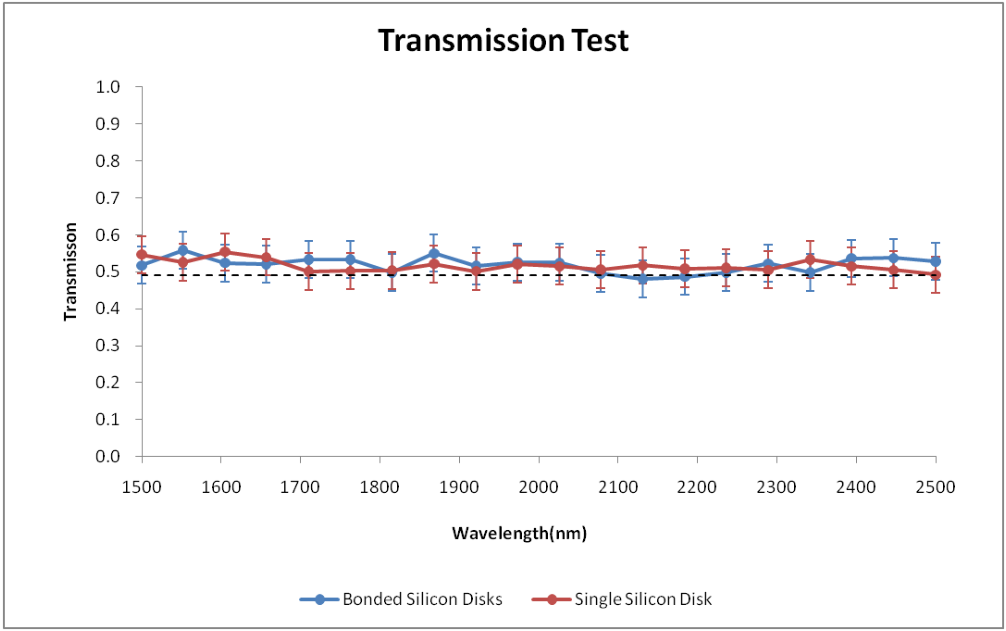
\psfig{file=chFabryPerot/HyeonjuTrans.pdf, width=\textwidth}
\caption[Hyeonju's transmission experiment]{Hyeonju's measurement of transmission as a function of wavelength for bonded Silicon pucks in the wavelength range $1500 < \lambda \textrm{(nm)} < 2500 $.  Hyeonju made the measurement with the CROWBAR on August 19, 2011.  The bonded Si pucks and double side polished reference puck show transmission indistinguishable within the uncertainty of the signal to noise $\sim5$ measurement.}
\label{fig:hyeonju-trans}
\end{center}
\end{figure}

\subsection{I modeled the Si$-$Air$-$Si gap as a Fabry-P\`{e}rot interferometer.}
I modeled the Si$-$air$-$Si gap as a Fabry-P\`{e}rot interferometer (also sometimes called an etalon).  There is a schematic of the cavity geometry below.  The key feature of a Fabry-P\`{e}rot is a cavity of length $L$ and refractive index $n$ separated behind two flat partially reflective surfaces with reflectivity $R$.  Light of wavelength $\lambda$ is incident at an angle $\theta$ to the normal of the cavity.  The cavity is characterized by the phase difference $\delta$ between the walls, which sets the (wavelength-dependent) output etalon transmission, $T_e$.  We also define the so-called ``coefficient of Finesse'', $F$.  Note that the ``coefficient of Finesse'' $F$ and the oft-used ``Finesse'' $\mathcal{F}$ are non-linearly related to each other, but here I will only employ the former $F$.
\begin{eqnarray}
 \delta = \frac{2\pi}{\lambda}2d \\
  F \equiv \frac{4R}{(1-R)^2} \\
 T_e = \frac{1}{1+F\sin^2(\delta/2)}  \label{eq:FabPerot}
\end{eqnarray}

\begin{figure}[h!] 
\begin{center}
\ 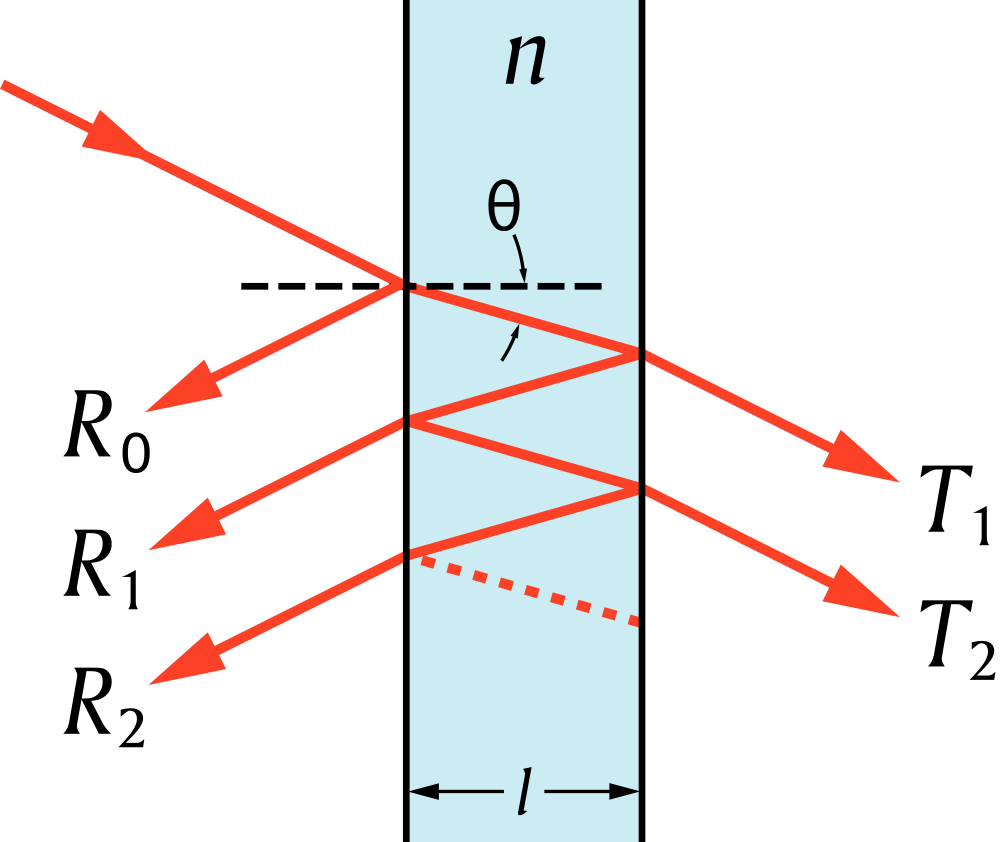
\psfig{file=chFabryPerot/Etalon.png, width=0.5\textwidth}
\caption[Etalon schematic]{Schematic of reflection and transmission at the interfaces of an etalon.  Our experiment involves an air gap sandwiched between two Si walls.  The reflectance of the Si walls originates from the sharp transition of refractive index, so called Fresnel reflection.  This figure is copied from Wikipedia, it is licensed under Creative Commons Attribution-ShareAlike 3.0 License by author Kevin Morse.}
\label{fig:etalon}
\end{center}
\end{figure}

I computed the wavelength-dependent reflection of the cavity sidewalls in the following way.  I first computed the wavelength-dependent refractive index from the Sellmeier equation for Si from the NASA Goddard CHARMS group\cite{2006SPIE.6273E..77F}.  The environment was room temperature (295 K).  I assumed the refractive index of air is 1.0.  I then used the equation for Fresnel reflection normal to an interface of media: 


where, importantly, the refractive index $n_{Si}=n(\lambda)$.  The Air$-$Si interface reflection $R$ ranges from 31.3\% to 30.1\% over the wavelength range 1100$-$3300 nm.  The coefficient of Finesse $F$ is about 2.66$-$2.46 over 1100$-$3300 nm.  $T_e$ is above 80\% for $\lambda > 1500$ nm for gap sizes of $L< 75$ nm.  For gaps of 125 nm the transmission through the cavity is merely 60\% at 1500 nm.  So, Hyeonju's measurement setup would not have been able to detect gaps smaller than about 75 nm.  A 125 nm gap was ruled out at 2$\sigma$.

\subsection{The Cary 5000 is 20$\times$ faster and more precise than CROWBAR.}

The Cary 5000 high performance UV-Vis-NIR spectrophotometer is 20$\times$ more sensitive, and about 20$\times$ faster than CROWBAR for straight-through transmission tests.  The Cary 5000 spectral range is 175$-$3300 nm, with at least 1 nm resolution.  The unit I have access to is housed at the UTexas Center for Nano and Molecular Science (CNM) on the UTexas main campus, room FNT 2.116.

\begin{figure}[h!] 
\begin{center}
\ 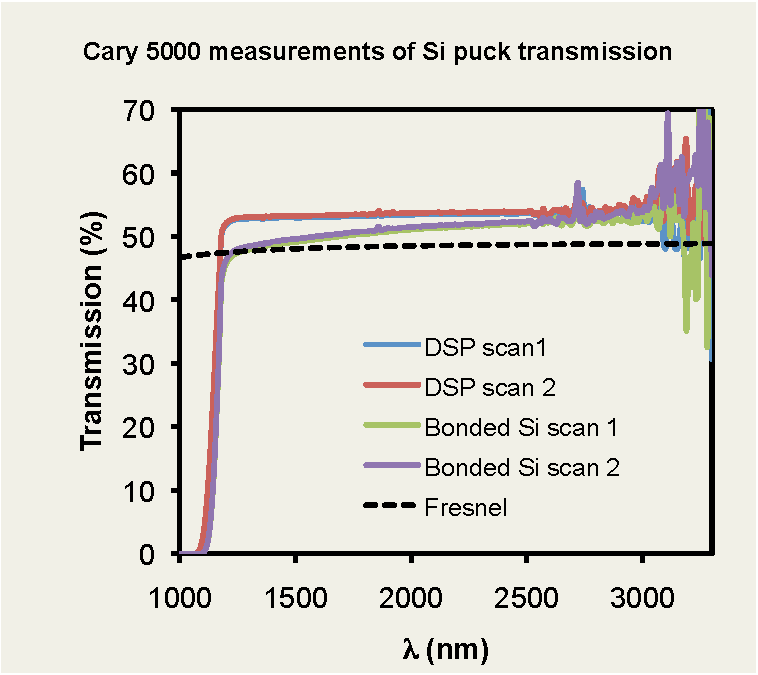
\psfig{file=chFabryPerot/Cary-gully-trans.pdf, width=0.88\textwidth}
\caption[Cary 5000 transmission]{Transmission of the bonded pucks HA1$-$HA2, the pucks Hyeonju Jeong bonded in 2011.  Also shown is a reference double side polished silicon puck.  Each piece was measured twice.  The repeated measurement lines are mostly indiscernible from the thick lines used for presentation on these high signal to noise ratio, high dynamic range measurements.  The transmission of the reference puck clearly differs from the bonded puck.  Atmospheric absorption degrades measurements at wavelengths greater than 2500 nm.  It is a mystery why the transmission exceeds the Fresnel prediction.}
\label{fig:Cary500}
\end{center}
\end{figure}


I measured the transmission of the DSP puck and the bonded pucks in the following way.  The lamp warmed up for 15 minutes.  I took a baseline scan with no optical elements in the beam path, but the holders and mounts were all in place.  Then I placed the DSP Si puck in the beam and took a scan.  The settings were single beam path, with 10 nm steps, with range 1000$-$3300 nm.  The scan took less than 5 minutes.  I replaced the DSP puck with the bonded Si puck.  I repeated the DSP puck and bonded puck measurements again, so the test order was `ABAB'.  The figure above shows the transmission as a function of wavelength for the four individual reference and target measurements.  The measurement repeatability is about 1 part in 300.  I estimated the repeatability by differencing the two scans and dividing by two (which is admittedly overestimating the repeatability by a factor of two).  I added the repeat scans and divided by two to estimate the average transmission.  The Si transmission cutoff is pretty conspicuous in the vicinity of $\lambda=1100$ nm.  

\subsection{I found evidence for an air gap in the bonded Si pucks.} 

It is clear that the transmission curves of the DSP and bonded Si pucks are different.  If the repeatability is a good estimate for the systematic errors, then individual data points on these curves are different by 6 $\sigma$ at 2200 nm and 13 $\sigma$ at 1400 nm.  I constructed the ratio of transmissions of the bonded Si pucks to DSP reference puck: $$T_{gap}=T_{bonded}/T_{DSP}$$  This ratio divides out the front and back Fresnel losses to reveal the transmission of the gap.  I compared this wavelength-dependent transmission to the Fabry-P\`{e}rot interferometer model transmission.  Below I plot the measured gap transmission ratio $T_{gap}$.  I under-plot three Fabry-P\`{e}rot model curves with different gap widths 30, 41, and 50 nm.  The gap is consistent with a 41 nm air cavity.

\begin{figure}[h!] 
\begin{center}
\ 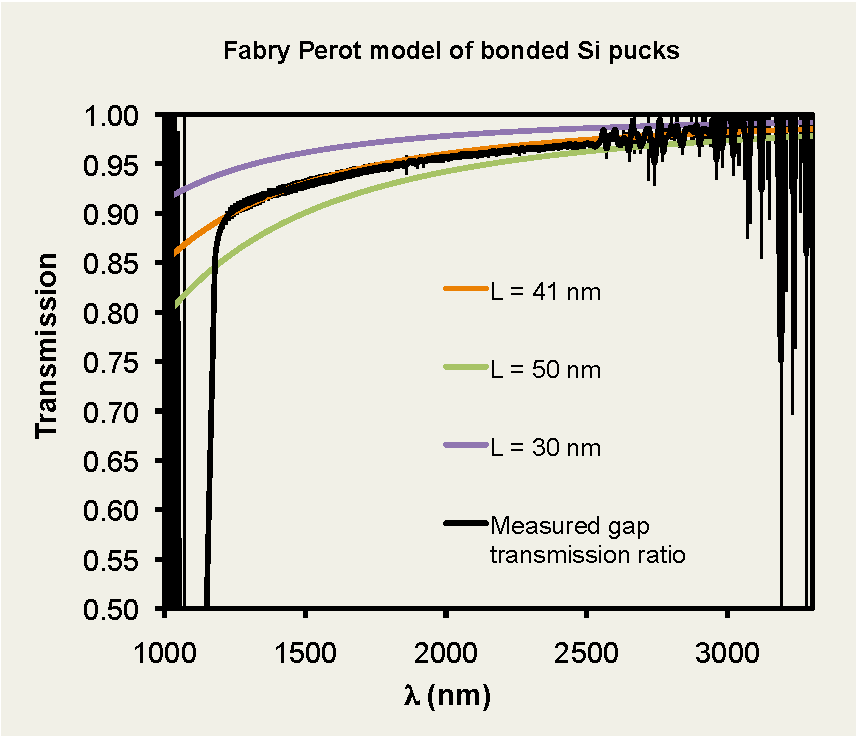
\psfig{file=chFabryPerot/FabPerot-gully-trans.pdf, width=0.92\textwidth}
\caption[Fabry-P\`{e}rot model of HA1$-$HA2]{Small ($<10\%$) transmission losses attributable to the gap are clearly distinguishable from measurement uncertainty.  Modeling of the gap as a Fabry-P\`{e}rot etalon with a uniform gap over the $\sim 12 \textrm{ mm } \times 20\textrm{ mm }$ area reveals an average gap size of 41 nm.  Models of 30 and 50 nm gaps are clearly rejected based on the measurement uncertainty.  The precipitous drop off at 1100 nm is from Si absorption.}
\label{fig:FabPerotHA1HA2}
\end{center}
\end{figure}


\section{Hyeonju's bonded Si wafers from 2010$-$2011}

I scrutinized four Si samples in the wavelength range 1100$-$2500 nm with 10 nm sampling with the Cary 5000.  I set the slit-width bandwidth (SWB) to 5 nm.  Last time I used the default 2 nm SWB.  I measured transmission in these samples:
\begin{enumerate}
  \item DSP Si wafer reference
  \item DSP Si puck HA1$-$HA2
  \item Hyeonju's bonded Si wafer A.  This was a whole 3 inch pair.
  \item Hyeonju's bonded Si wafer B.  This was a wafer shard.
\end{enumerate}

\begin{figure}[h!] 
\begin{center}
\ 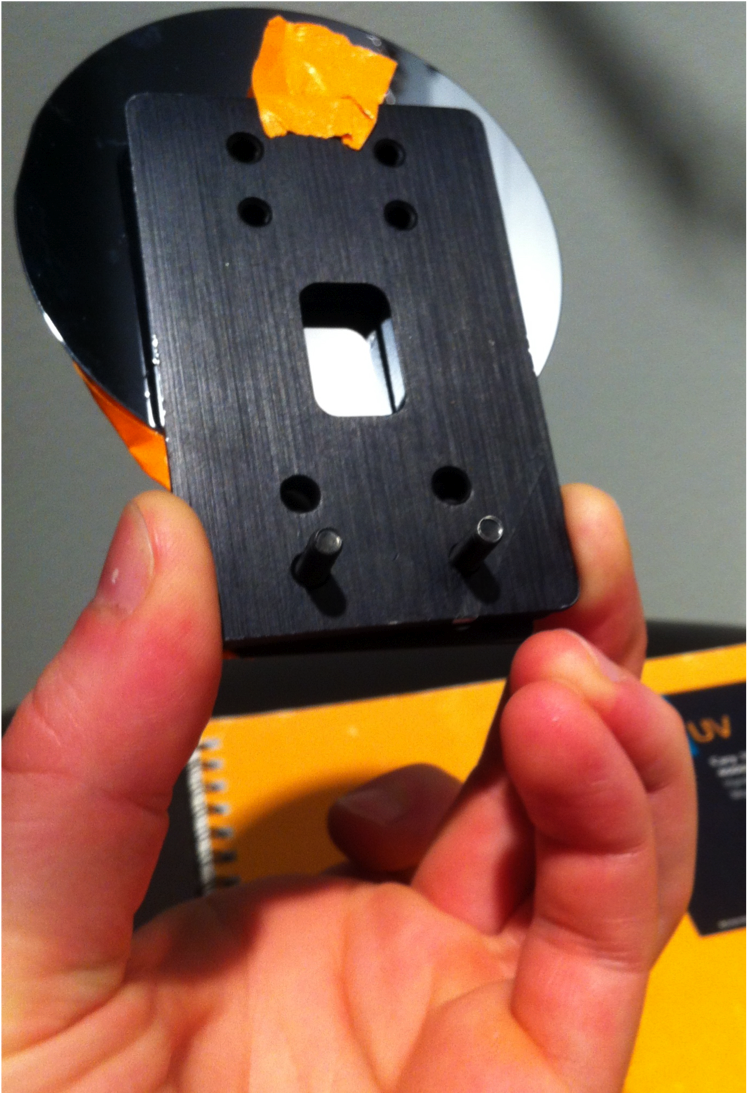
\psfig{file=chFabryPerot/bonded-wafer-holder-pic.png, width=0.5\textwidth}
\caption[Cary 5000 sample size]{A photo of the Cary 5000 sample holder.  The area is about 12 mm $\times$ 20 mm.  At the time of writing it is not known if the beam is uniform over that area.  Hyeonju's bonded Si wafer A is taped to the sample holder.}
\label{fig:Cary5000sampleArea}
\end{center}
\end{figure}

\subsection{The measurement repeatability is about 1 part in 200.}

I tested the transmission of a 7 mm thick reference DSP Si puck on Monday and Wednesday.  The median difference between individual transmission measurements over the wavelength  was 1 part in 200.  The median difference between individual transmission measurements taken between Monday and Wednesday was 1 part in 100.


\begin{figure}[h!] 
\begin{center}
\ 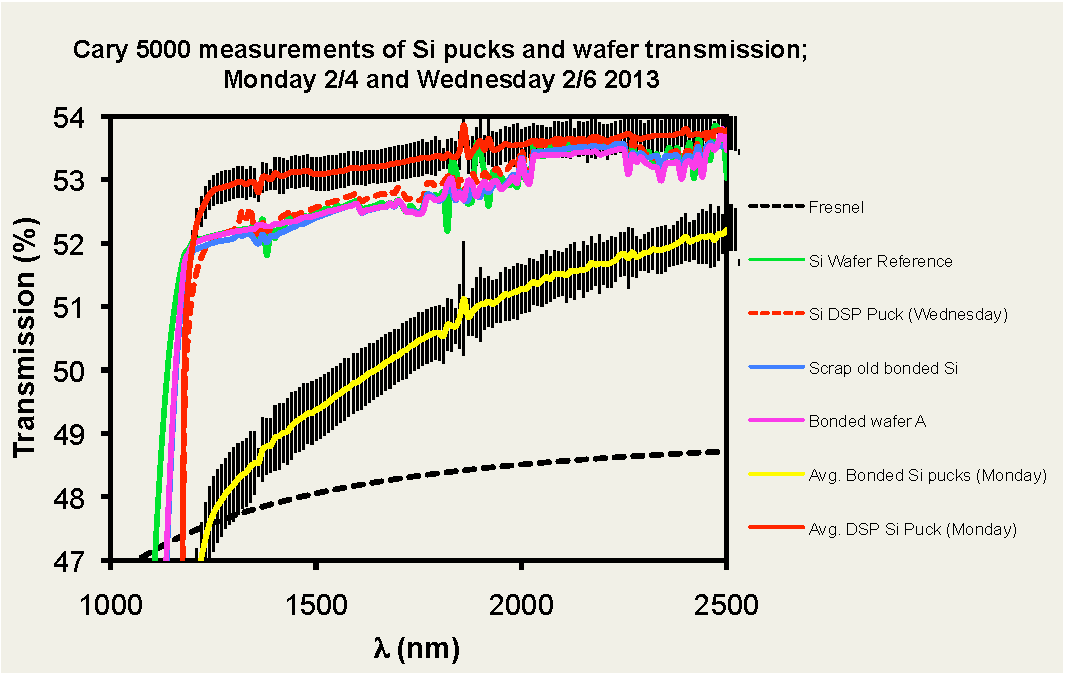
\psfig{file=chFabryPerot/gully-Si-wafers-transmission.pdf, width=1.0\textwidth}
\caption[Bonded Si wafer transmission]{This graphic demonstrates a few key aspects of our measurements, which I will describe the in order of magnitude of the effect.  First, the transmission of Si wafers exceeds the prediction for Fresnel reflection (dashed curve) by 5\% (i.e. 10\% of the $\sim$50\% signal, or about 20$\sigma$).  This discrepancy is a mystery, we speculate about its origin in later sections.  Second, the bonded wafer puck is clearly separated from the DSP reference samples.  Third, the systematic error from repeatability from two different days is perceptible by the top red curve and its companion dashed red curve a half percent below.  Lastly, all the wafers, whether bonded or not, demonstrate indistinguishable transmission properties, which is evidence for negligible gap in the bonded wafers.}
\label{fig:Cary5000wafer}
\end{center}
\end{figure}

\subsection{I found no measurable difference between the transmission of bonded wafers and DSP wafers.}

All the transmission curves of bonded and non-bonded Si wafers lie within the measurement error of each other, as seen in the figure below.  We can put an upper limit on the gap width with our Fabry-P\`{e}rot model.  We construct the transmission of the gap the same way we did last time, namely we divide the transmission of the bonded Si wafers by the transmission of the DSP wafer.  I construct the uncertainty as the standard deviation of all four transmission measurements.  The median uncertainty is 0.002.  Recall that the gap widths I report assume that the gap is air.  If the gap is some higher index material, then the gap widths could be larger.  With that proviso, a gap width of 4 nm or less is consistent with the bonded Si wafer transmission.  A gap width of 12 nm is ruled out at over 5$\sigma$.


\begin{figure}[h!] 
\begin{center}
\ 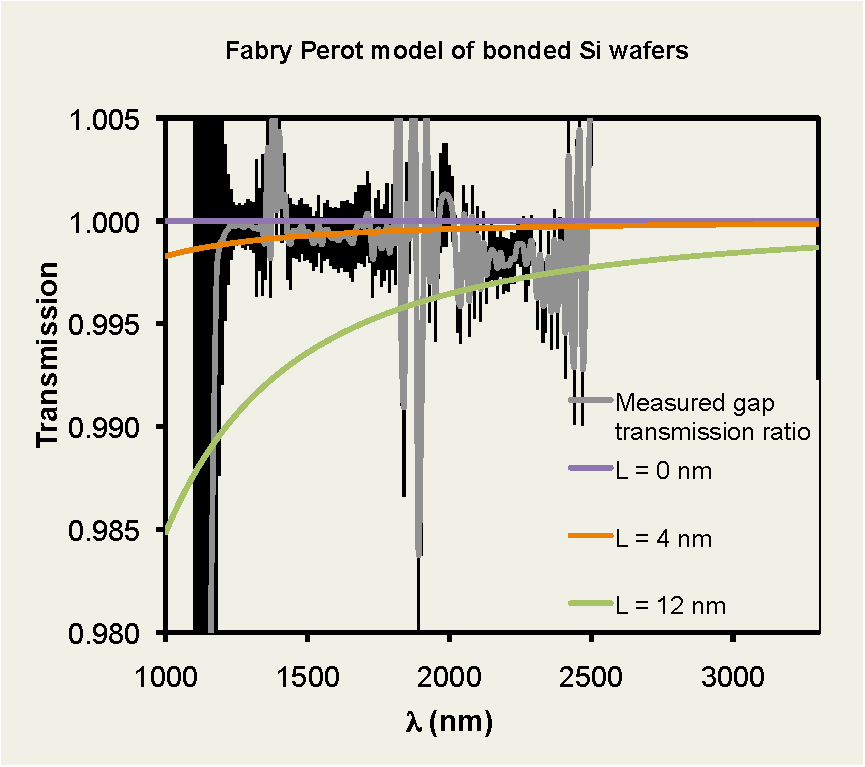
\psfig{file=chFabryPerot/gully-Si-wafers-fabperot.pdf, width=1.0\textwidth}
\caption[Fabry-P\`{e}rot model shows $<4$ nm gaps in wafers]{The average measured transmission of bonded Si wafers compared to three Fabry-P\`{e}rot models for air gaps of 0, 4, 12 nm.  A gap width of 12 nm is ruled out at over 5$\sigma$.}
\label{fig:Wafers4nmGap}
\end{center}
\end{figure}


\section{JPL Microdevices Lab fabrication and metrology of gaps of known size}

I begin this section by describing experiments conducted during my visit to the NASA JPL Microdevices Lab (MDL) on February 11$-$15, 2013.  I predict the transmission curves for bonded Si disks and wafers with known gap sizes.  I present the measured transmission curves and interpret the observations.  Finally I conclude with a summary and recommendations for moving forward.

\subsection{I characterized the surfaces of 7 thick Si substrates.}

Victor White (NASA JPL Microdevices Lab) had 7 thick Si substrates with uncertain heritage.  I recorded the peak to valley surface error and shapes over the center 2 inch diameter for all substrates, front and back when available.  The tool is a Fisba2.  I recorded surface roughness with Wyko 2D optical profiler.  The five DSP 3.3 mm thick 4'' diameter substrates exhibited between 0.3$-$0.8 waves per surface, with a ``Pringle'' or ``saddle'' morphology.  The surface roughness was 5.0 nm RMS over a 1 mm sq. area.  Two DSP Virginia Semiconductor 15 mm thick, 3'' diameter pucks, exhibited 0.9$-$3.5 waves peak to valley, with a convex sphere shape.  A reference Si wafer exhibited 1.2 nm RMS roughness over a 4.6 $\times$ 3.5 mm area.  The peak to valley roughness is about 5 times the RMS roughness.  

\subsection{Substrate preparation is multifaceted.}

The substrate preparation was multifaceted.  We start with ultrasonic cleaning in acetone for about 5 minutes, immersion rinse in methanol and IPA, then `Megasonic' (GHz frequency ultasonic) rinse for 5 minutes in DI water, and N$_2$ airgun for 1 minute.  We performed MHz frequency O$_2$ plasma ashing.  The pieces cooled.  We sprayed them with DI water, followed by blow dry for 10 seconds and then stuck the pieces together.  We applied pressure in the center by hand with clean gloves.  The parts were inseparable when I tried shearing the parts with moderate human strength.

\subsection{We made two bonded Si wafers and two bonded Si pucks.}

Victor and I made two bonded Si wafers and two bonded Si pucks, labeled as VG01$-$VG04 in the table below.  VG02, VG03, and VG06 are the five DSP substrates that all exhibited a ``saddle'' morphology on their surface.  VG01, VG04, and VG05 are special ordered 1 mm thick wafers with two flats angled at 45$^\circ$ to each other.  The packaging of VG02, VG03, and VG06 indicates the resistivity is 6.11$-$8.19 ohm-cm with CZ growth process; I do not have this information for the 1 mm thick wafers.  The wafers and pucks are all 100 mm diameter, except for VG05, which is cleaved into two equal-sized halves.  We keep a DSP single wafer (VG05) and puck (VG06) to serve as transmission references with identical properties as their bonded counterparts.

\begin{center}
    \begin{tabular}{ c c c c c c c}
    \hline
    Name & Bonded/DSP & Type & Thickness & Flats & Date & Notes \\ 
        \hline
    VG01 & Bonded & Wafers & $1$ $\times$ 2 mm & Two; 45$^\circ$ & 2/13/2013 &  \\
    VG02 & Bonded & Pucks & $3.3$ $\times$ 2 mm & Two, 90$^\circ$  & 2/13/2013 &  \\
    VG03 & Bonded & Pucks & $3.3$ $\times$ 2 mm & Two, 90$^\circ$ & 2/14/2013 & 4 $\mu$m hole \\    
    VG04 & Bonded & Wafers & $1$ $\times$ 2 mm &  Two; 45$^\circ$ & 2/14/2013 & 15 nm gap \\        
    VG05 & DSP & Wafer & 1 mm &  Two; 45$^\circ$ & 2/15/2013 & cleaved  \\
    VG06 & DSP & Puck & 3.5 mm &  Two, 90$^\circ$ & 2/15/2013 & \\
    \hline
    \end{tabular}
\end{center}

\subsection{We found initial evidence for a gap.}

Victor and I placed the pieces in a vintage IR Suss mask aligner. This vertically mounted aligner has an IR blub, sample holder, microscope objective, and an IR detector (Victor guessed J-band wavelength range).  We basically did Hyeonju's ``method 1'' test. Namely, we focused on the front surface then the back surface, recorded the vertical position of the objective, then went to the middle to look for features in the bond.  We did not see any high spatial frequency structures (i.e. dust), but it was hard to distinguish the front and back surfaces on the 6 mm stack of Si. We noticed a large scale transmission variation across the bonded thick disks.  This transmission variation is consistent with a Fabry-P\`{e}rot air cavity inside.

\subsection{We made a gap of known dimension.}

Bonded parts VG03 and VG04 have gaps of known dimensions.  For VG03 we made a cylindrical hole on the surface of one puck with the following technique.  We spin-coated a conventional thick photoresist on the surface of the puck.  We exposed the resist to a UV lamp with a photomask bearing a flower-leaf pattern on a predominantly dark mask.  We exposed a $\sim$1'' diameter circle of light on top of the flower-leaf pattern so that the latent image looked like a sunflower with a big clear area in the center.  After clearing the exposed resist we plasma etched the silicon with SF$_6$ for about 4 minutes.  Dektak stylus profilometry indicated that the etch depth was 4.0 $\mu$m.  We contacted the side with the hole to the inside of the silicon bonded system so that it was trapped in the gap.  I mapped out where the gap was with the IR Suss mask aligner, marking the location of the hole with a permanent marker.  The figure below shows a schematic of the VG03 pattern.

\begin{figure}[h!] 
\begin{center}
\ 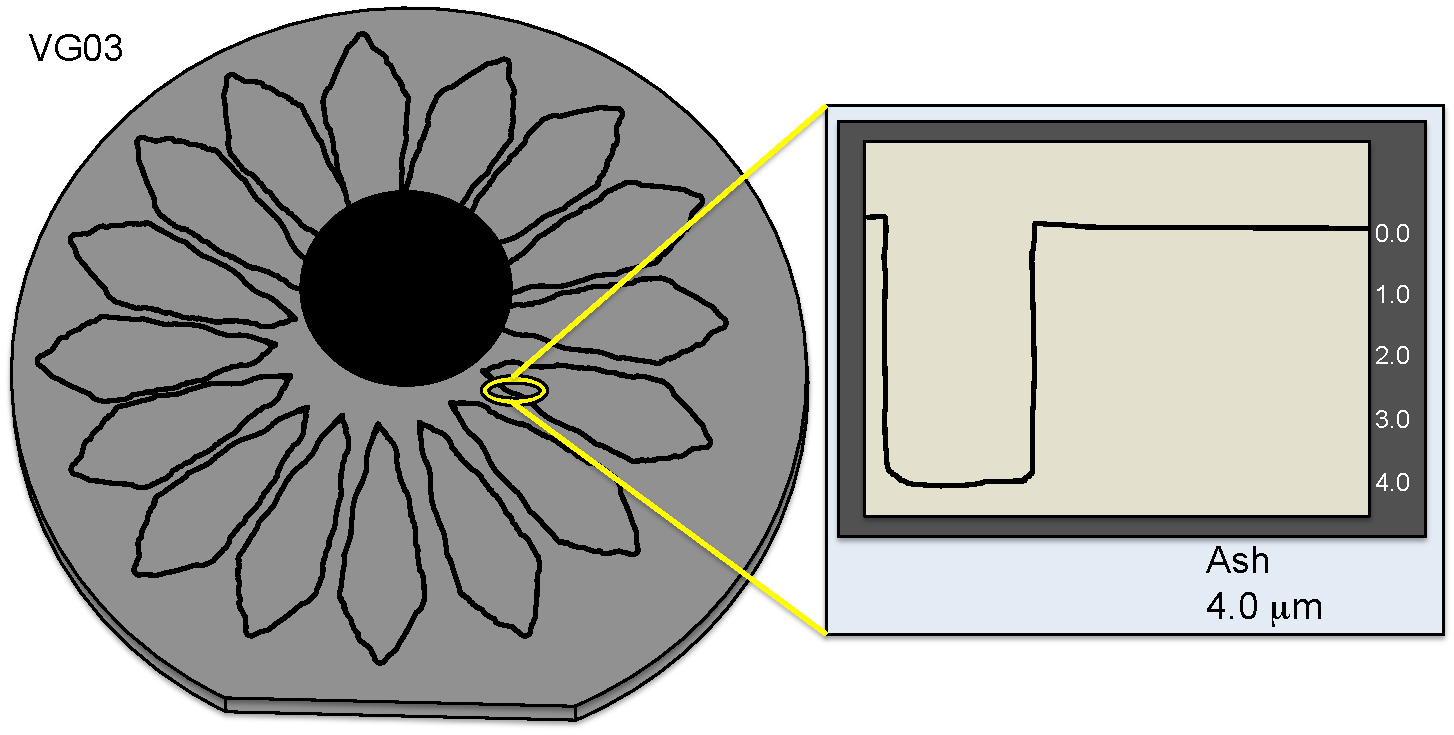
\psfig{file=chFabryPerot/VG03_pattern.pdf, width=0.82\textwidth}
\caption[VG03 Pattern]{This is a detail of the pattern on the surface of VG03.  The depth is about 4000 nm.}
\label{fig:VG03pattern}
\end{center}
\end{figure}


VG04 was prepared in a similar way as VG03.  We patterned VG04 with a resolution test mask which has many tiny features on the order of 1 mm to sub-micron scales.  We do not know the fill factor at the time of writing, but the mask is mostly clear, with perhaps only 20\% chrome by area.  The fill factor is important to us so we will have to characterize the pattern after the fact.  The pattern size was $\sim$1'' diameter circle. After development we performed a plasma etch with CHF$_3$ for a few minutes.  We measured the etched depth with a Veeco/Wyko 2D non-contact interferometer microscope.  We achieved a depth of about 15 nm.  Unfortunately, we did not mark the pattern boundary.  The pattern is roughly in the center.  We predict the gap to behave like a Fabry-P\`erot cavity.  Since we know the gap sizes we can predict how the air gap transmission spectrum should behave. 

\begin{figure}[h!] 
\begin{center}
\ 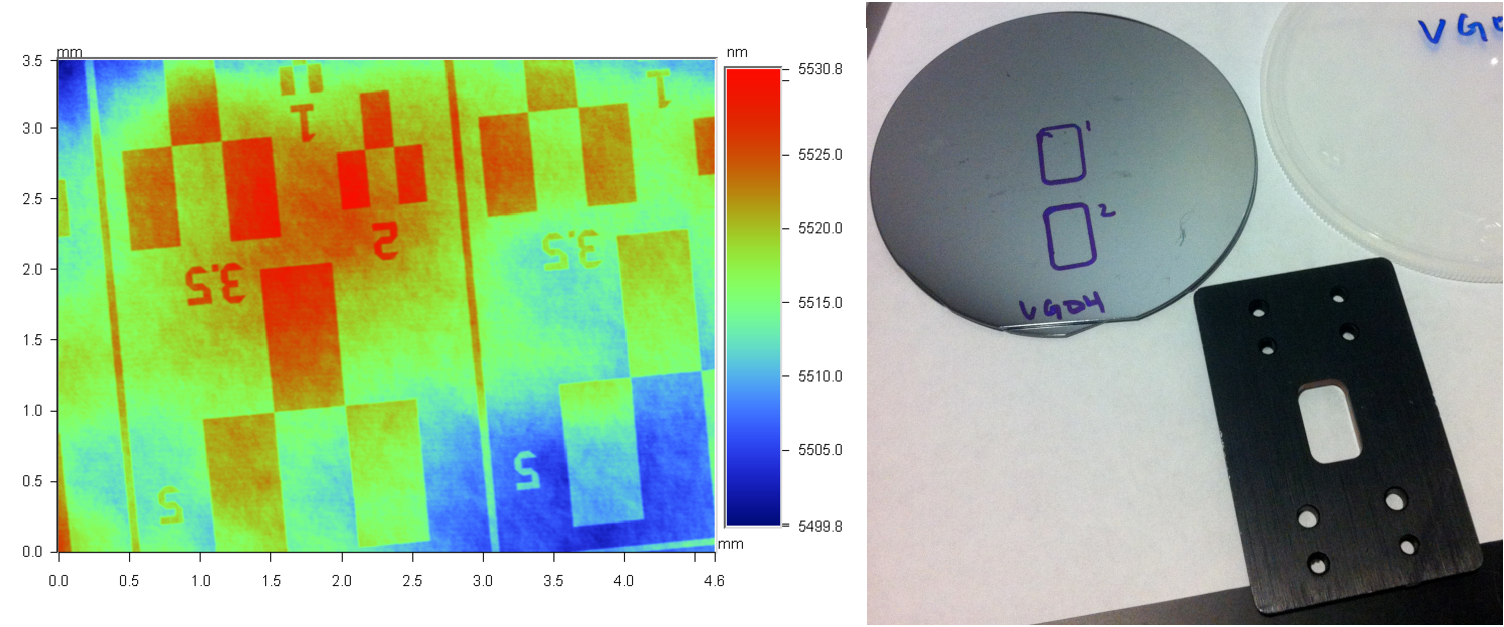
\psfig{file=chFabryPerot/VG04_detail.pdf, width=\textwidth}
\caption[VG04 Detail]{Detail of the pattern and its location in VG04.  Measurement locations are marked 1 and 2 in the photo at the right.  Position 1 is roughly at the location of the of the pattern, while position 2 is in an area that should be fully contacted (no gaps). }
\label{fig:VG04detail}
\end{center}
\end{figure}

\subsection{Transmission measurements are consistent with gaps.}

\begin{center}
    \begin{tabular}{c c c}
    \hline
    Measurement \# & Target & Time \\ 
        \hline
       0& Baseline 100\%T  & 2:21:48 PM \\
       1 &Baseline 0\%T  & 2:24:52 PM\\
       2 &VG05  & 2:30:16 PM\\
       3 &VG01  & 2:34:12 PM\\
       4 &VG06  & 2:40:46 PM\\
       5 &VG02 Pos 1  & 2:45:16 PM\\
       6 &VG02 Pos 2  & 2:49:21 PM\\
       7 &VG02 Pos 3  & 2:53:58 PM\\
       8 &VG02 Pos 4  & 2:57:52 PM\\
       9 &VG03 Pos 1  & 3:02:22 PM\\
      10& VG03 Pos 2  & 3:06:13 PM\\
      11 &VG04 Pos 1  & 3:12:33 PM\\
      12 &VG04 Pos 2  & 3:16:32 PM\\
      13 &VG06 post  & 3:24:42 PM\\
      14 &Baseline 100\%T  & 3:28:57 PM\\
      15 &Baseline 0\%T  & 3:31:56 PM\\
      16 &VG05 post  & 3:35:34 PM\\
    \hline
    \end{tabular}
\end{center}

I measured the transmission as a function of wavelength with the Cary 5000 UV-Vis-NIR spectrophotometer on February 18, 2013.  I took a dark scan and a baseline scan before and after.  There was a 2\% increase in the baseline scan intensity over a time period of 71 minutes.  The baseline drift is probably from lamps warming up and flicker noise and so forth.

\begin{figure}[h!] 
\begin{center}
\ 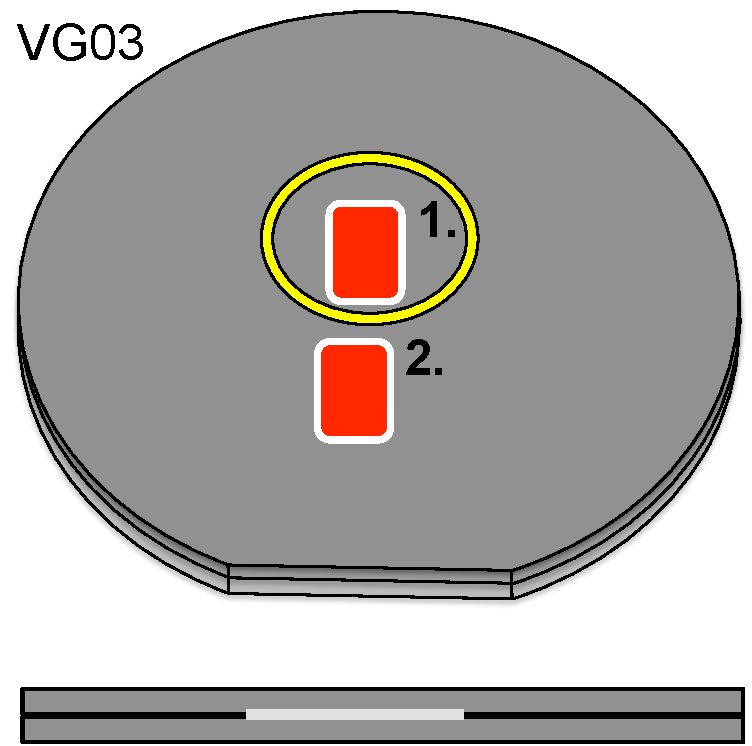
\psfig{file=chFabryPerot/VG03_PDF.pdf, width=0.5\textwidth}
\caption[VG03 Schematic]{We marked the location of the 4000 nm divot with a permanent marker while it was imaged with the IR mask aligner.  We are confident that the measurement box was fully encapsulated in the divot.}
\label{fig:VG03schematicl}
\end{center}
\end{figure}

Below I show plots of the transmission for part VG03.  The measured values are a dotted black line.  My strategy to correct for drift was to normalize the etalon transmission by the average of two scans of VG06 which occurred 20 minutes before and after.  In this way, any linear drift term should be averaged out.  I took two scans of VG03 separated by 4 minutes, in two different positions as shown in the schematic above.  Position 1 is on the gap and position 2 is on what should be a contacted region.  

\begin{figure}[h!] 
\begin{center}
\ 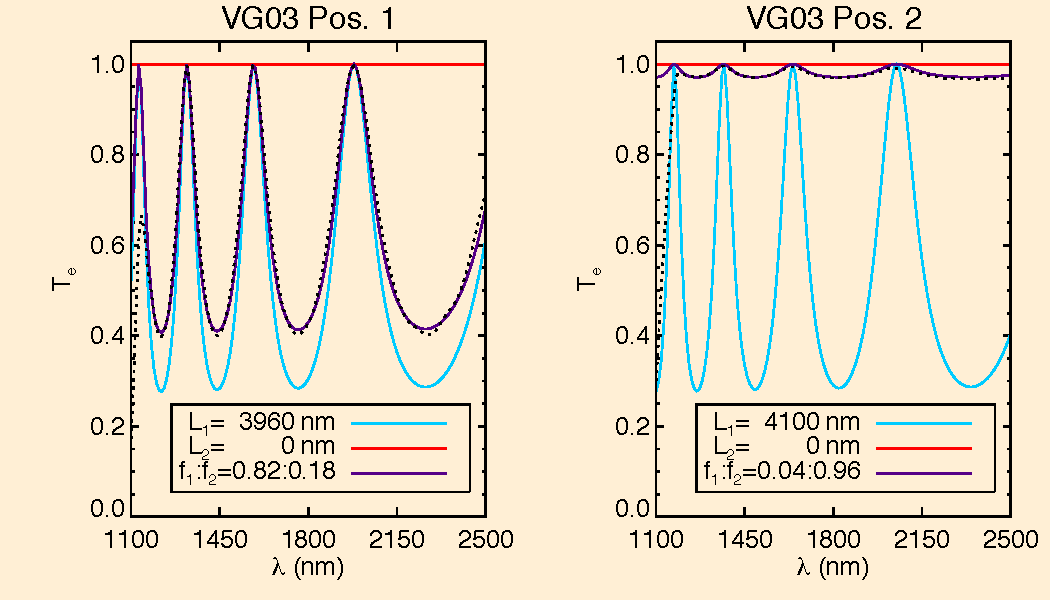
\psfig{file=chFabryPerot/VG03_1and2.pdf, width=0.95\textwidth}
\caption[VG03 Transmission]{Transmission spectra of VG03 in positions 1 and 2.}
\label{fig:VG03transl}
\end{center}
\end{figure}

The transmission spectrum at position 1 is consistent with a 3960 nm gap with 18\% of the measurement area fully contacted (zero gap).  Position 2 is consistent with a 4100 nm gap covering only 4\% of the measured area.  The 4\% must be the flower-leaf petal lines, which take up a small area, but are deep troughs. 

\begin{figure}[h!] 
\begin{center}
\ 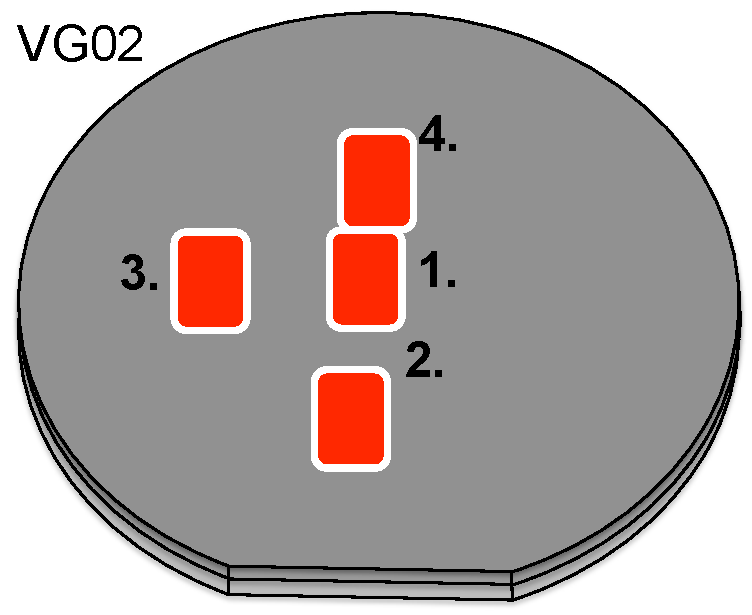
\psfig{file=chFabryPerot/VG02.pdf, width=0.5\textwidth}
\caption[VG02 measurement position layout]{Measurement layout of VG02}
\label{fig:VG02layout}
\end{center}
\end{figure}

\begin{figure}[h!] 
\begin{center}
\ 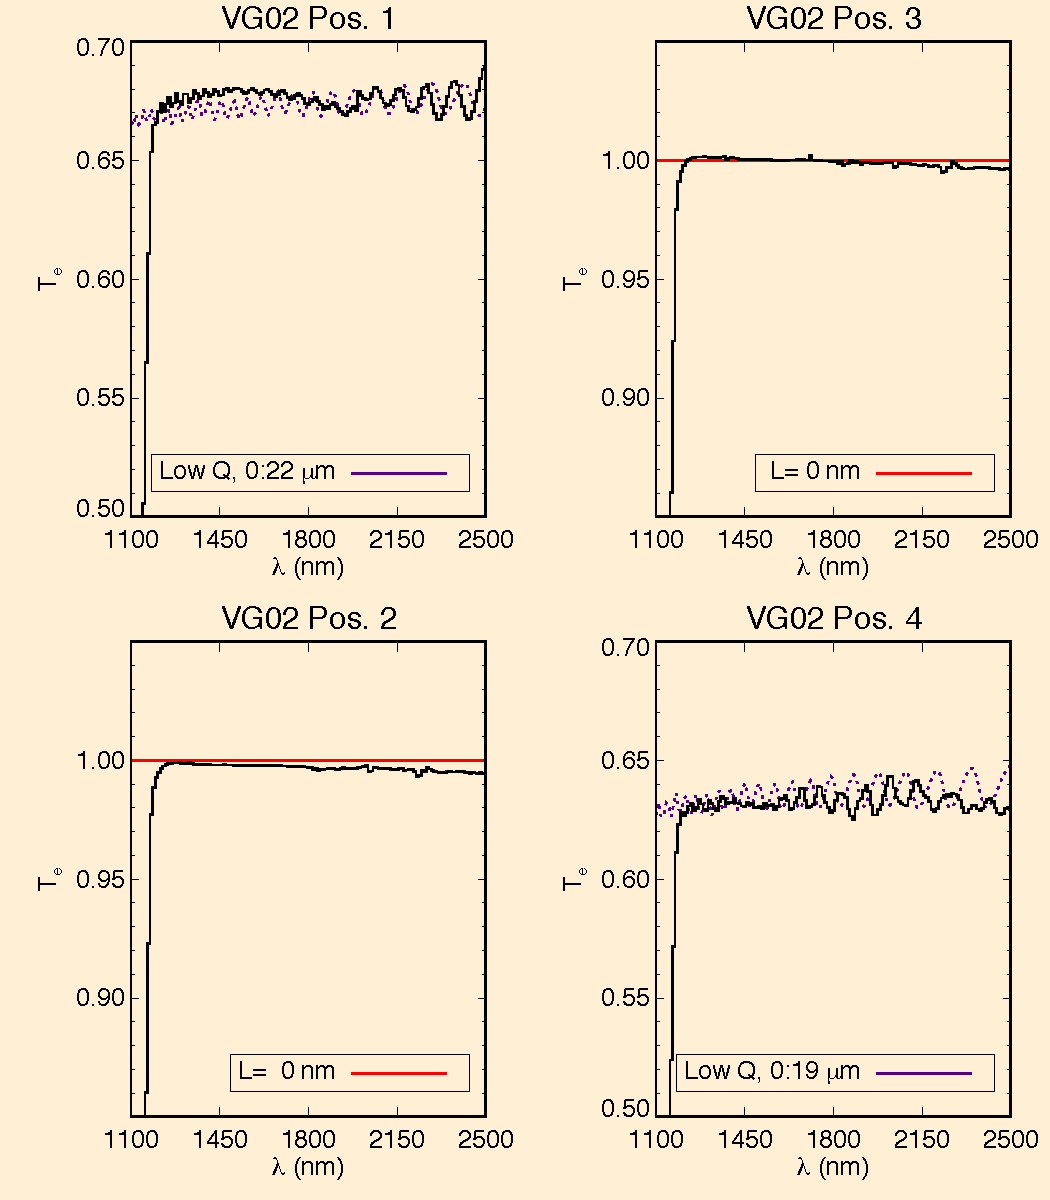
\psfig{file=chFabryPerot/VG02_1to4.pdf, width=0.95\textwidth}
\caption[VG02 transmission in 4 position]{Transmission as measured in 4 distinct sub-apertures of VG02.}
\label{fig:VG02trans}
\end{center}
\end{figure}


I measured VG02 in four different positions as shown in the schematic above.  The transmission spectrum for positions 1$-$4 are shown.  Positions 2 and 3 are consistent with no or negligible cavity.  There is a systematic uncertainty of about 1 part in 200 because the baseline scans were not repeated close enough in time.  Specifically, the reference sample VG06 was measured 17 minutes before VG02 position 4, which is enough time to cause systematic drift.  Suffice it to say that better care could be taken to reduce the systematic error below 1 part in 200, but for now we will not attempt to correct the data beyond the automatic baseline and reference puck division.  I suspect that the systematic dip from 1900$-$2500 nm would go away with a better baseline scan.  Otherwise, the measurement could be consistent with a very small ($<1$\%) area possessing a 500 nm gap, although formal modeling was not attempted.  Positions 1 and 4 are different.  Positions 1 and 4 show an almost flat transmission profile with 67\% and 63\% transmission, respectively.  Close scrutiny of the transmission spectra reveal that the transmission oscillates around the average value with a peak to valley amplitude of about 1\%.  It is clear that these features are real, since the near-contemporaneous scans of position 2 and 3 demonstrate no such spectral fringes, as evinced in the identically scaled plots (all four plots cover 20\% of y$-$scale dynamic range).  I thought about how combinations of transmission profiles could reproduce a flat curve.  I tried a simple two stepped model with half the area at 100 nm and half at 500 nm.  I tuned the gap size and relative area, and could not achieve such a near spectrally flat profile, nor could I produce the fringes.  

So I constructed a so-called ``low$-$Q'' model, which I describe here.  The low$-$Q models are shown in purple dashed lines on top of the black lines, the data.  The low$-$Q model has a range in gap sizes.  The simplest version is a linear distribution of gap sizes, characterized by a smallest gap and a largest gap.  Physically, this model corresponds to a gap geometry that looks like a ``lean-to tent'' or a skateboard ramp.  There is a ground floor which is bonded, then some ramp, perhaps with a flat top.  More complicated models can be constructed by including more or fewer steps of the high or low gap, or making the ramp concave or convex.  I compute the model with a finite number $N$ of steps of different gap widths $L_i$ in the range $L_{min} < L_i < L_{max}$:

$$T_{LQ}= \sum_{i=1}^N \frac{1}{N}T_e(\lambda,L_i)$$

The frequency and amplitude of the wiggles and the average transmission constrain the Low-Q model.  The frequency of the wiggles sets the maximum gap width: higher measured fringe frequency means you need to include a larger peak gap size.  The amplitude of the wiggles sets the distribution of area weighted to the higher or lower gap width.  One way to think of this is a histogram of gap spacings: what fraction of the area exhibits gaps in different interval ranges.  The average transmission also constrains the distribution of area weighted to the higher or lower gap width, specifically what fraction of the area is is consistent with 0 gap width.  The interpretation of the model is degenerate since we only constrain what fraction of the area is at the higher or lower value, and not where these areas are spatially located with respect to each other, so we cannot distinguish between a pyramid or a quonset hut geometry, although in principle these disparate geometries would have different gap size distribution histograms.  In reality the distribution histogram is not very well constrained.  Besides, the better way to approach this problem is simply to take measurements with finer spatial resolution, namely by stopping down the aperture, or using alternative methods for imaging the bond.  

For VG02 position 1 we find that the spectral fringe frequency is best fit by a peak gap size of about 22.0 $\mu$m, with 30\% of the area contacted, and a weighting towards larger gap sizes.  We construct a histogram of the fraction of area at different heights, assuming the measurement beam is uniform, and the beam size is 1.2 cm $\times$ 1.6 cm = 1.9 cm$^2$ = 190 mm$^2$.  This area measurement is a coarse estimate at the time of writing.  For VG02 position 4 we conclude a peak gap size of 19$\mu$m, with 22\% of the area contacted, and the same distribution of weighting towards larger gap sizes as shown in the histograms.  Recall the proviso that these parameters are only weakly constrained, although I have not quantified that adequately here, it is not worth getting into that since there are better, non-degenerate ways to attack this question.  


\begin{figure}[h!] 
\begin{center}
\ 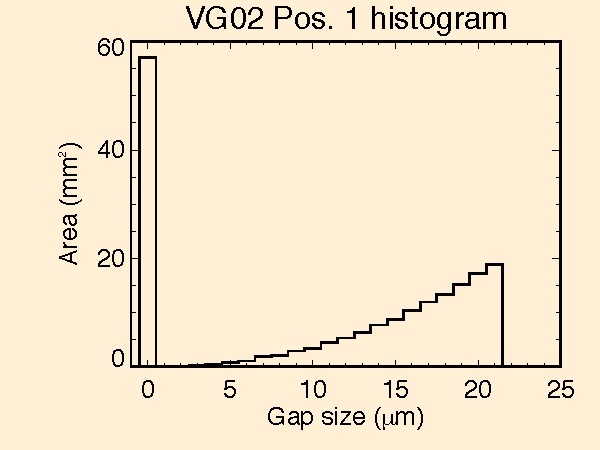
\psfig{file=chFabryPerot/VG02_pos1hist.pdf, width=0.48\textwidth}
\ 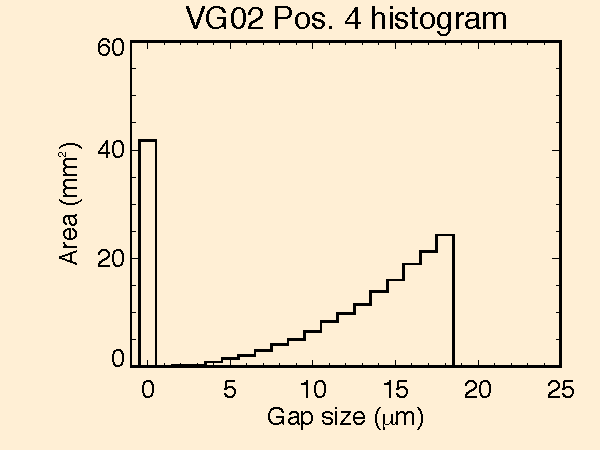
\psfig{file=chFabryPerot/VG02_pos4hist.pdf, width=0.48\textwidth}
\caption[VG02 gap size distribution]{A gap size distribution consistent with the measured transmission spectrum of VG02 positions 1 and 4}
\label{fig:VG02gapDist}
\end{center}
\end{figure}

So far we have examined VG02 and VG03, which were the two pairs of Si pucks we bonded.  Let's now turn to VG01 and VG04, which are the Si wafers Victor and I bonded.  I measured VG01 in the center, it is consistent with no gap, as shown in the figure below.

\begin{figure}[h!] 
\begin{center}
\ 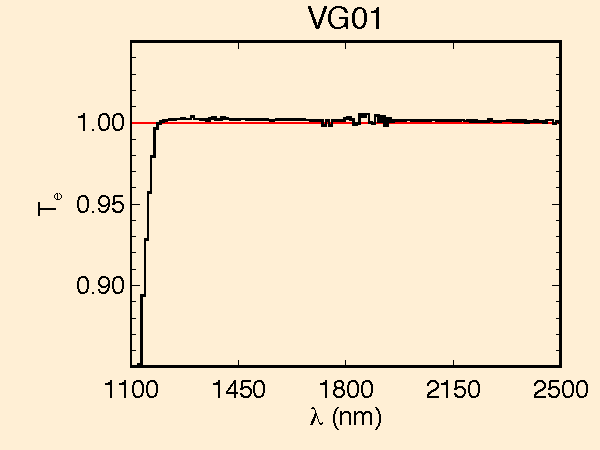
\psfig{file=chFabryPerot/VG01.pdf, width=0.65\textwidth}
\caption[VG01 transmission]{Measured transmission of VG01 is consistent with no, or negligible air gap.}
\label{fig:VG01trans}
\end{center}
\end{figure}

I measured VG04 in two areas shown in previous figures.  The black holder is shown in the photo, with the rectangular aperture clearly visible.  There are four small pesky holes that I had not covered up during the time of the measurement.  It is possible that light can go through the small holes and goof up the measurements.  I'm not sure, but in the future whoever performs the measurements should naturally cover up the holes with metallic or otherwise opaque tape.  The left side of the figure shows a detail of the pattern etched into the surface of one of the inside of the silicon wafers.  The vertical scale on the right side of the figure has a relative dynamic range of 5500 to 5530 nm.  The largest features there are basically 10$-$15 nm tall, and about 1.0 mm $\times$ 0.5 mm wide.  The patterned area is about 1 inch diameter, roughly in the center of the wafer.

The figure below shows the transmission in the two areas.  Position 2 is consistent with zero gap.  Position 1 is not well modeled with a two-component model, specifically the measurement between 1150 nm and 1300 nm diverges from the two component model shown in the figure.  A low$-$Q model was not attempted.  In any case, it is clear that the expected 25 nm gap is overwhelmed by a much large gap on the order of 550 nm.  I thought of another explanation, which is that the patterns are so small that they diffract light out of the measurement direction and so we perceive a reduction in transmission attributed to a Fabry-P\`erot etalon.  I have not done the calculation to rule this in or out.

\begin{figure}[h!] 
\begin{center}
\ 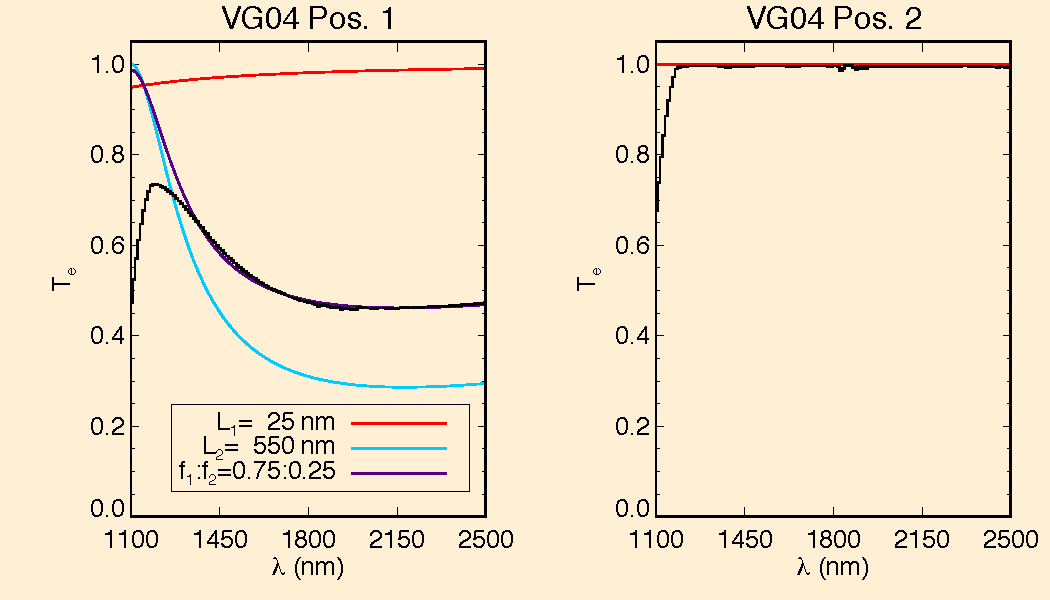
\psfig{file=chFabryPerot/VG04.pdf, width=0.85\textwidth}
\caption[VG04 transmission]{Measured transmission of VG04 demonstrates a larger gap ($\sim550$ nm) than anticipated ($\sim15-25$ nm).  }
\label{fig:VG04trans}
\end{center}
\end{figure}

\subsection{Why does the observed transmission exceed the Fresnel prediction?}

One outstanding question is why the measured transmission exceeds the prediction from Fresnel reflection.  The plot below summarizes the problem.  The dashed lines are repeat measurements of DSP silicon wafers, which lie well above the predictions for two air$-$Si reflections.


\begin{figure}[h!] 
\begin{center}
\ 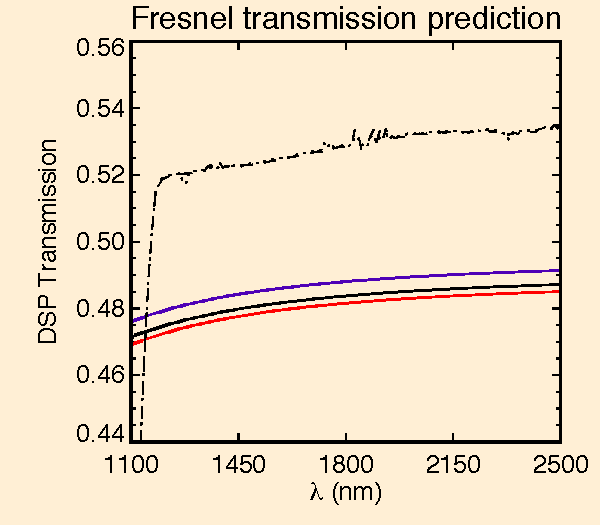
\psfig{file=chFabryPerot/fresnel_Si_index.pdf, width=0.5\textwidth}
\caption[Fresnel prediction]{The Fresnel prediction for Si transmission is 90\% of the transmission measured.  The discrepancy persists despite any unreasonable estimate of temperature.  It would take changing the Si refractive index to an unreasonable value of about 3.2 in order to boost the post-dicted Fresnel transmission model to the observed value.}
\label{fig:Fresneldiscrepancy}
\end{center}
\end{figure}


I looked into this question in one specific way.  I looked at how the transmission scales with temperature of Silicon.  The temperature enters in because the refractive index, $n$, depends on temperature; the Air$-$Si interface reflection, $R$, depends on the refractive index; the coefficient of finesse, $F$, depends on the reflection; and the etalon transmission, $T_e$, depends on the finesse.  I constructed the refractive index for $T=\;77, \;295, \;373$ K, and computed the etalon transmission for a gap size of 4100 nm.  I used the temperature dependent refractive index from Frey et al. 2006.  Notably, I extrapolated their curves to 373 K, for which no measurements were available.  Our measurements occur near room temperature, probably 295 $\pm$ 3 K.  From 295 K to 77 K the refractive index changes only by a maximum of 0.92\% in the wavelength range 1100 to 2500 nm.  The concomitant etalon transmission changes only by 0.3\% for a gap size of 41 nm.  For a 4100 nm gap, the peak fractional difference in etalon transmission is 1.5\%.  The figure below shows the model for a 4100 nm gap- the etalon transmission curves are indistinguishable with the thickness of the lines shown.  A mere hint of a difference can be seen in the valleys of the transmission minima.  The figure demonstrates that the tiny refractive index differences expected for normal room temperature variations will be vastly less than any measurement error.


\begin{figure}[h!] 
\begin{center}
\ 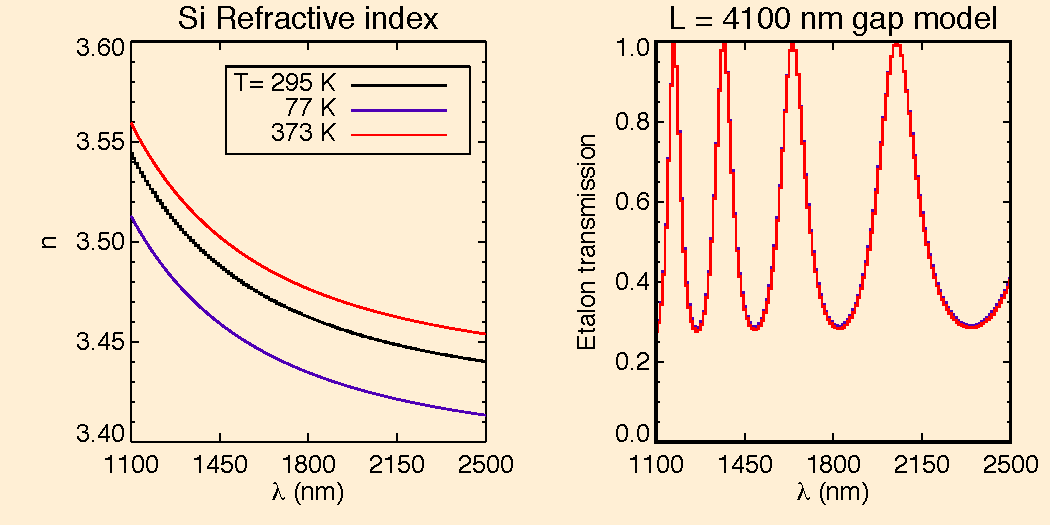
\psfig{file=chFabryPerot/Si_index_temp, width=\textwidth}
\caption[Si temperature has negligible effect on Fabry-P\`{e}rot]{The ambient temperature will have no measurable impact on the Fabry-P\`{e}rot transmission.}
\label{fig:SiTempFP}
\end{center}
\end{figure}

\textbf{Summary, and the path forward}

The table below summarizes the outcome of the bonding experiments and IR transmission metrology.  

\begin{center}
    \begin{tabular}{ c c c c}
    \hline
    Name & Predicted Gap & Measured Gap & Interpretation \\ 
        \hline
    VG01 & 0 nm & 0 nm & Wafers seem to bond very well \\
    VG02 & 0 nm & 0$-$22 $\mu$m & Glove speck wedged in the gap during contact\\
    VG03 & 4.0 $\mu$m & 4.0 $\mu$m  & As expected, affirms the Fabry$-$P\`erot model \\    
    VG04 & 10$-$25 nm & 550 nm &  The pillar-pattern may inhibit bonding \\        
    \hline
    \end{tabular}
\end{center}

\section{Efforts to make the metrology and bonding more robust.}

There are a few problems we still have to solve to make the metrology and bonding more robust.

\subsection{Is the difference between predicted and observed transmission attributable to oxide acting as an anti-reflection coating?}
First, we must explain why the air$-$Si interface transmission measurement and prediction disagree far outside the measurement error.  One disputed explanation is that a tiny oxide layer on the surface acts as a weak anti-reflection coating.  Oxide grows naturally on Silicon at room temperature at atmospheric pressure.  The layer is thin, of order 1 nm.  The refractive index of SiO$_2$ is 1.46.  We can get a handle on the magnitude of the purported transmission loss of an AR coating by modeling the layer with two different techniques already familiar from this chapter- scalar Fresnel theory and Fabry-P\`erot theory.

The Fresnel strategy is to treat the air$-$SiO$_{2}-$Si transition as a cascade of air$-$SiO$_2$ and SiO$_{2}-$Si layers, each with transmission dictated by the Fresnel loss at an interface of different refractive indices.  This technique is independent of the thickness of the oxide thin film.  The technique is almost certainly inappropriate for sub-wavelength scales, but probably would work for gaps much larger than the wavelength.  Specifically, the interference effects inside the oxide layer are probably important.  I proceed anyways just to see what the magnitude of the effect would be if this technique were appropriate.  I computed the transmission using equation \ref{eq:Fresnel}, updated for the index pairs of air$-$SiO$_2$ and SiO$_{2}-$Si.  The reflection at these interfaces is about 0.035 and 0.16, respectively.  I computed the transmission through each interface and multiplied the transmissions together to get a single side transmission.  I squared the single side transmission to get the net double side polished transmission $T_{AR}$ of an oxide AR coating.  I found a value of $T_{AR}=0.652$.  Contrast $T_{AR}$ to our original Fresnel prediction for a cascade of two air$-$Si interfaces $T_{Si}=$0.487, and our measured value of 0.53-0.54 (depending on the wavelength).  The silicon dioxide AR coating model is incompatible with the measured transmission values.  However, an AR coating of a different refractive index would satisfy the measured transmission.  I calculated the two refractive indices at which the modeled transmission would fall in the range 0.53-0.54.  Values of  3.11$<n<$3.16 and 1.085$<n<$1.105 satisfy the measured transmission.  There is viable candidate material with these ranges of refractive index.  Instead, the material could be a surface-roughened hybrid combining silicon and air, silicon and oxide, silicon and air, or some mixture of all three interfaces.  This scheme is likely if the roughness is significantly sub-wavelength so that light just ``sees'' the hybrid layer effectively as a single layer of intermediate index.  The effective index would most likely be a pure arithmetic mean of the two indices.  No pair of indices of silicon, air, or oxide have arithmetic means in the vicinity of 3.1 nor 1.1.

Another strategy is to model the oxide layer as a Fabry-P\`erot, with the oxide layer serving as the cavity.  This strategy has the problem that the cavity walls have unequal reflection coefficients, $R$.  Specifically the reflection at the air$-$SiO$_2$ interface is 0.035 and the reflection at the SiO$_{2}-$Si interface is 0.16.  The standard Fabry-P\`erot summation of interfering plane waves is incompatible with unequal reflections, since the forward- and backward- reflected plane waves will have incomplete cancellation.  Accordingly, calculating the Finesse is not straight-forward.  Despite this challenge we can still estimate a bound the magnitude of the transmission through the oxide cavity by trying two values of Finesse- one calculated for $R_{low}=0.035$ and one with $R_{high}=0.16$.  We assume a gap spacing in the range 0.1$-$10 nm, which is sufficiently liberal to  capture any reasonable value for oxide film thickness, which I've measured with ellipsometry to be about 1 nm for similarly prepared Si substrates.  I employed equation \ref{eq:FabPerot}, updated for the oxide refractive index.  I calculated the net transmission for a double side polished Si wafer by squaring the calculated etalon AR coating transmission since the front and back interfaces contribute equally.  The strongest decrement will occur for the shortest wavelength ($\lambda$ = 1200 nm), with the highest Finesse ($R_{high}=0.16$), with the largest assumption for the gap (10 nm).  Under these extreme conditions the decrement is merely 99.8\%, which is negligible.  More realistic estimates for the gap yield transmissions closer to unity.  Furthermore, the direction of Fabry-P\`erot interference is always to decrease (or leave unchanged) the transmission.  The measured DSP Si transmission is always \emph{higher} than the predicted Fresnel transmission.  So we can conclusively rule out Fabry-P\`erot interference attributable to a purported oxide layer on Silicon.  
 
An experimental method is to remove the oxide layer with an HF dip then remeasure the piece.  Along the same lines, we must explain why the troughs in the spectral fringes of VG03 do not get to as low a transmission as we would expect.  Increasing the air$-$Si surface reflection would also resolve this latter problem, so the oxide layer explanation has a second thread of support.  Surface roughness could also mimic an AR coating, but this explanation is unlikely because the surface roughness is so different in the wafers and the pucks, yet we see the same performance in transmission.  

What if the Cary 5000 UV-Vis-NIR detector is non-linear?  Typically NIR detectors are non-linear in the sense that the wells fill up faster when they are empty (low signal), then accumulation becomes less effective when the wells are closer to full ( 

\subsection{Strategies for improving the spatial resolution of transmission test}
Second, we seek more spatial information on the bond geometry.  Specifically we wish to develop a technique that can provide the gap size over $x-y$ scales of less than a few square millimeters, so we have hundreds or more spatial elements over the whole 4'' diameter circular area.  The morphology of the bond gap may give us clues as to what is causing gaps- for example isolated dust specks, or large scale surface deformation.  I am recommending that we experiment with monochromatic IR lasers in transmission.  Monochromatic techniques suffer from an $n\lambda/4$ degeneracy, so this technique must either be reserved for gaps everywhere less than $\lambda/4$, or the technique can be coupled with a coarsely dithered transmission spectrum.  The figure below shows the expected etalon transmission as a function of gap size for $\lambda \;= \;1523$ nm. 

\begin{figure}[h!] 
\begin{center}
\ 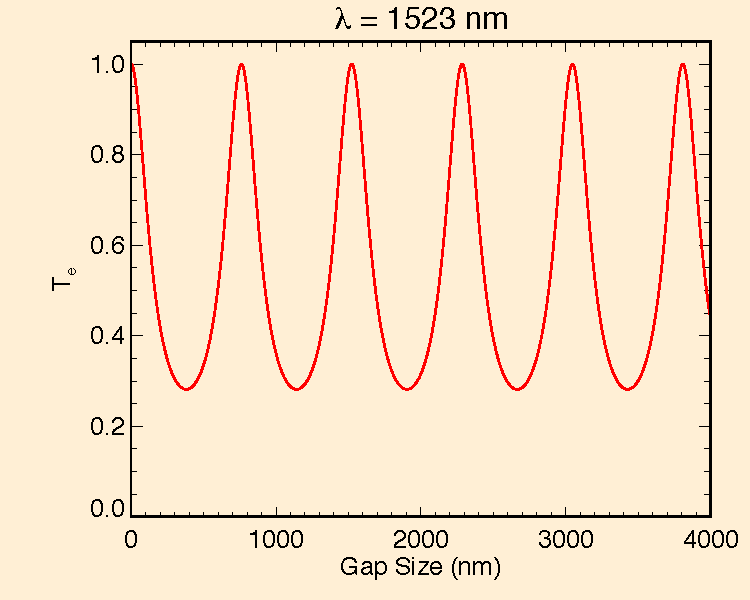
\psfig{file=chFabryPerot/1523_fabperot.pdf, width=0.8\textwidth}
\caption[Monochromatic Fabry-P\`{e}rot at 1523 nm]{Expected transmission as a function of gap size for a fixed wavelength- a 1523 nm HeNe laser.}
\label{fig:1523nmFP}
\end{center}
\end{figure}

\subsection{Can we implant and detect tiny ($\sim$20 nm) gaps?}
We would still like to demonstrate that we can faithfully recover small (i.e. few to tens of nanometer) gaps with the Fabry$-$P\`erot transmission spectrum technique. VG04 demonstrated a much larger gap than expected (550 nm vs 15$-$25 nm), possibly because the pillar-pattern inhibited the bond front propagation, but really we don't know.  We will have to devise other ways of inserting tens of nanometer size gaps.  Dan Jaffe suggests making a pattern in the shape of the bio-hazard symbol, or an array of boxes that are sunken-in.  These patterns may allow the bond front to zipper around the features.  Another promising strategy is to employ vendor-provided nano-spheres or microspheres.  

\subsection{To what extent will initial Si surface morphologies comply during bonding?}
I am recommending that we keep track of the orientation and surface properties of surfaces before bonding.  Specifically, we should have full aperture interferometry and roughness measurements of the surfaces before bonding, and track relative orientation of morphological features.  In this way we can see if the same morphologies arise in high-spatial resolution metrology of the bond cavity.  For example if both surfaces have a convex ``focus'' morphology, we may expect that the centers will be in firm contact and the outside will demonstrate a tiny cavity.  It would be nice to predict the morphology of gaps based on a-priori interferometry.  If we see these morphologies in bonded pieces then we might conclude that we did not apply enough force during contacting to deform the surfaces.  

\subsection{Can we use ellipsometry to probe the gaps?}
I am still interested in testing out ellipsometry as a way to probe the cavity.  I am interested in monitoring the bond-front propagation in-situ, with either an IR camera like the Suss, or a transmission spectrum technique.

\subsection{Runs \#4 and \#5 characterize the Cary 5000 tool performance.}

\begin{center}
    \begin{longtable}{c c c c c  c}
    \caption[Cary 5000 run \#4 and \#5]{Experiment log for the Cary 5000 UV-Vis-NIR spectrophotometer} \label{CaryRun4-5} \\

    \hline
     \# & ID & Time & Aperture & Angle & Note\\ 
    \hline
     \endhead

\hline \multicolumn{6}{c}{{\emph{Continued on next page}}} \\ \hline
\endfoot

\hline \hline
\endlastfoot

        \hline
       \multicolumn{6}{c}{Run \#4-- May 2, 2013} \\
         \hline
       0 & Baseline 100\%T &  10:41:23 PM  & none & 0$^{\circ}$ & \\
       1 & Baseline 0\%T &   10:44:29 PM  & black & - & \\
       2 & run\_03 &   10:52:32 PM  &12$\times$20 mm & - & Holes covered\\
       3 & run\_04 &   10:56:09 PM  &12$\times$20 mm & - & Holes uncovered\\
       4 & run\_5 &   11:00:07 PM  & 12 mm & - & Holes taped over\\
       5 & Baseline 100\%T &   11:03:11 PM  & none & - & \\
       6 & Baseline 0\%T &   11:06:30 PM  & black & - &  \\
       7 & run\_6 &   11:09:56 PM  & 10 mm & - & \\
       8 & run\_7 &   11:13:37 PM  & 8 mm & - & \\
       9 & run\_8 &   11:18:28 PM  & 5 mm & - & \\
      10 & Baseline 100\%T &   11:21:26 PM  & none & - & \\
      11 & Baseline 0\%T &   11:24:20 PM  & black & - & \\
      12 & run\_9 &   11:27:24 PM  & 4 mm & - & \\
      13 & run\_10 &   11:30:59 PM  & 2 mm & - & \\
      14 & run\_11 &   11:35:02 PM  & 1 mm & - & \\
      15 & Baseline 100\%T &   11:38:42 PM  & none & - & \\
      16 & Baseline 0\%T &   11:41:32 PM  & black & - & \\
      17 & run\_12 &   11:45:16 PM  & 12$\times$20 mm & - & ND filter \# 1\\
      18 & run\_13 &   11:49:10 PM  & 12$\times$20 mm & - & ND filter \# 2\\
      19 & run\_14 &   11:53:11 PM  & 12$\times$20 mm & - & ND filter \# 3\\
      20 & run\_15 &   11:56:41 PM  & 12$\times$20 mm & - & ND filter \# 4\\
              \hline
       \multicolumn{6}{c}{May 3, 2013} \\
               \hline
      21 & run\_16 &   12:00:28 AM  & 12$\times$20 mm & - & ND filter \# 5\\
      22 & Baseline 100\%T &   12:03:20 AM  & none & - & \\
      23 & Baseline 0\%T &   12:06:12 AM  & black & - & \\
      24 & run\_17 &   12:09:17 AM  & 12$\times$20 mm & - & ND 2,3\\
      25 & run\_18 &   12:13:00 AM  & 12$\times$20 mm & - & ND 2,3,4\\
      26 & run\_19 &   12:16:24 AM  & 12$\times$20 mm & - & ND 2,3,4,5\\
      27 & run\_20 &   12:20:30 AM  & 12$\times$20 mm & - & ND 2,3,4,5,1\\
      28 & Baseline 100\%T &   12:23:48 AM  & none & - & \\
      29 & Baseline 0\%T &   12:26:39 AM  & black & - & \\
      \hline
       \multicolumn{6}{c}{Run \#5-- May 3, 2013} \\
      \hline
      30 & Baseline 100\%T &    12:22:17 PM & none & 0$^{\circ}$& \\
      31 & run\_21 &    12:26:48 PM & none & 0$\pm$3$^{\circ}$& VG05\\
      32 & run\_22 &    12:31:11 PM & none & 10$\pm$3$^{\circ}$ & VG05\\
      33 & run\_23 &    12:35:30 PM & none & 20$\pm$3$^{\circ}$ & VG05\\
      34 & Baseline 100\%T &    12:38:35 PM & none & 0$^{\circ}$& VG05\\
      35 & run\_24 &    12:42:29 PM & none & 30$\pm$3$^{\circ}$& VG05\\
      36 & run\_25 &    12:46:19 PM & none & 40$\pm$3$^{\circ}$ & VG05\\
      37 & run\_26 &    12:49:54 PM & none & 50$\pm$3$^{\circ}$ & VG05\\
      38 & run\_27 &    12:53:49 PM & none & 60$\pm$3$^{\circ}$ & vignetting, VG05\\
      39 & Baseline 100\%T &    12:59:21 PM & none &0$^{\circ}$ & \\
      40 & run\_28 &    1:03:24 PM & none & 0$^{\circ}$& blank measurement\\
      41 & Baseline 100\%T &    1:06:24 PM & none & 0$^{\circ}$&\\
      42 & run\_29 &    1:09:56 PM & none & 0$^{\circ}$& blank measurement\\
      43 & Baseline 100\%T &    1:16:13 PM & none & 0$^{\circ}$& \\
      44 & run\_30 &    1:19:37 PM & none & 30$\pm$3$^{\circ}$& VG03 pos 1\\
      45 & run\_31 &    1:23:57 PM & none & 0$\pm$3$^{\circ}$& VG03 pos 1\\
      46 & Baseline 100\%T &    1:34:40 PM & none & 0$^{\circ}$& \\
      47 & run\_32 &    1:37:57 PM & 12$\times$20 mm & 0$^{\circ}$& VG03 pos 1\\
      48 & run\_33 &    1:42:51 PM & 12 mm & 0$^{\circ}$& VG03 pos 1\\
      49 & run\_34 &    1:46:41 PM & 10 mm & 0$^{\circ}$& VG03 pos 1\\
      50 & run\_35 &    1:50:39 PM & 8 mm & 0$^{\circ}$& VG03 pos 1\\
      51 & run\_36 &    1:55:29 PM & 5 mm & 0$^{\circ}$& VG03 pos 1\\
      52 & run\_37 &    1:59:45 PM & 4 mm & 0$^{\circ}$& VG03 pos 1\\
      53 & Baseline 100\%T &    2:02:57 PM & none & 0$^{\circ}$& \\
      54 & run\_38 &    2:06:58 PM & 2 mm & 0$^{\circ}$& VG03 pos 1\\
      55 & run\_39 &    2:12:23 PM & 2 mm & 0$^{\circ}$& VG03 pos 1 redo\\
      56 & run\_40 &    2:15:47 PM & 2 mm & 0$^{\circ}$& blank\\
      57 & Baseline 100\%T &    2:19:13 PM & none & 0$^{\circ}$& \\
    \hline
    \end{longtable}%\end{tabular}
\end{center}

\subsection{Raw signal, artifacts, and instrumental characterization}
The raw signal from the Cary 5000 100\% baseline scan  is shown in Figure \ref{fig:Cary5000baseline}.  The details of the raw signal largely do not matter, since the baseline serves as the normalization of all subsequent measurements.  There are two subtle features to notice.  There is a factor of 10 in dynamic range, so measurements at longer wavelengths will generally have lower signal to noise ratios than those at shorter wavelength.  The Cary 5000 has a constant signal to noise ratio operation mode that I have not explored.  The second important feature of the raw spectrum is the large jumps in signal strength between different hardware configurations.  The spectral locations of the jumps is listed in the table below.  

\begin{figure}[h!] 
\begin{center}
\ 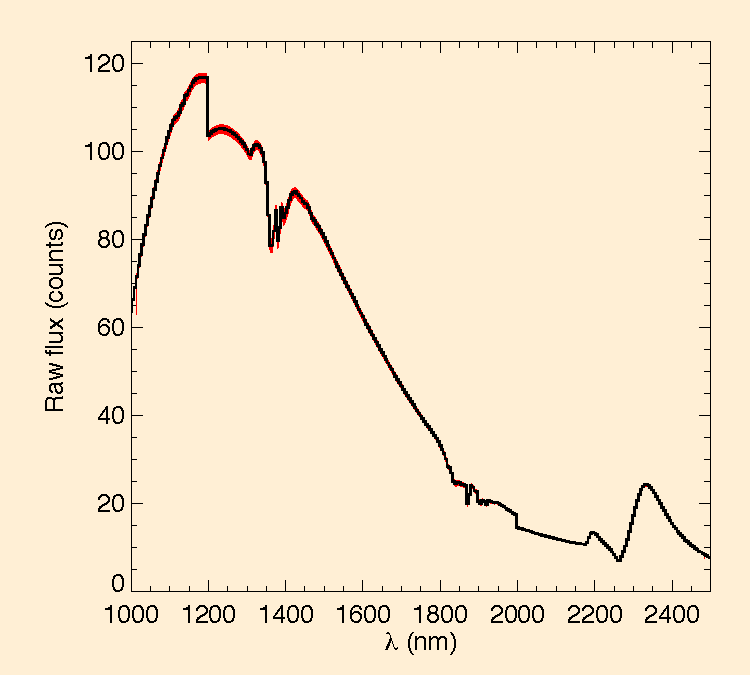
\psfig{file=chFabryPerot/20130502_baseline.pdf}
\caption[Cary 5000 raw spectrum]{Raw spectrum of the Cary 5000.  The black line is the mean of six 100\% baseline scans sampled over 2 hours.  The red filled band defines the maximum and minimum bounds at each spectral sample.}
\label{fig:Cary5000baseline}
\end{center}
\end{figure}

\newpage
1
\newpage
1
\newpage
1

\begin{longtable}{lc}
    \caption[Cary 5000 Characterization]{Cary 5000 characterization and operational properties} \label{tab:C5000Char} \\

    \hline
     Property (units) & Value \\ 
    \hline
       Spectral sampling interval (nm) & 5 \\
       Single measurement bandwidth (nm) & 5 \\
       Time per sample (s) & 0.1 \\
       Available measurement range (nm) & 175$-$3300 \\
       Typical measurement range (nm) & 1000$-$2500 \\
       Number of samples per spectrum & 301 \\
	Standard deviation of a single measurement (\%) & 0.02 \\
	Peak to valley deviation of a single measurement (\%) & 0.2 \\
	Overall scale error per measurement (\%) & 0.16 \\
	Lamp drift over 2 hours (\%) & $0.7-2.5$ \\
	Mean 0\% baseline magnitude (\%) & 0.03 \\
	Beam profile & \emph{rectified Gaussian} \\
	Beam FWHM (mm) & 5 \\
	\multirow{2}{*}{Wavelengths of known instrumental artifacts (nm)} &  \\
      &1200 \\
      &1350 \\
      &1360$-$1450\\
      &1850 \\
      &1800$-$1950 \\
      &2000 \\
      Vendor-reported linearity range (dB) & 40 \\
      Directly measured linearity range (dB) & $>24$ \\
    \hline
\end{longtable}

\newpage


\subsection{Does spurious light get through the screw holes in the Cary 5000 sample holder?}
Figure \ref{fig:Cary5000sampleArea} shows a photo of the Cary 5000 12 mm $\times$ 20 mm sample holder aperture.  This sample holder aperture serves as the pupil stop in the collimated beam of polychromatic light.  The sample holder is opaque over most of its surface except for the center aperture and 8 screw holes for sample mounting.  I simply adhere silicon samples to the sample holder, usually with double sided carbon sticky tape.  This mounting strategy could suffer from scattered light passing through the screw holes and diluting the spectra with unintended spurious spectra.  The fraction of area open to the screw holes is about 20\% that of the center aperture, so any putative spurious signal could be significant contributor to systematic error.

I can rule out spurious light from the screw holes as a contributor to our measurement error.  The signal attributable to light passing through the screw holes has a mean value of 0.1\% of the signal, which is comparable to the 0.16\% uncertainty attributable to overall scale shifts per measurement.   

\subsection{Beam size}
We would like to know the Cary 5000 beam size.  Measurements of the spurious signal through the screw holes in the previous section coarsely constrains the beam size to much less than the roughly 40 mm spacing of the screw holes on the sample holder.  The largest vendor-provided aperture is 12 $\times$ 20 mm.  The smallest vendor provided aperture is a pinhole less than 1 mm in diameter.  I fabricated 7 custom aperture plates intermediate in size between the vendor provided apertures.  The apertures are 2'' $\times$ 2'' square aluminum, about 1 mm thick.  I drilled circular holes in the center of the square apertures.  The drill bit diameters defined the circle diameters.  No chamfering was performed; the extent of kerf loss is unknown.  The seven diameters are 12, 10, 8, 5, 4, 2, and 1 mm.  

Experiments named ``run\_5'' through ``run\_11'' were aimed at characterizing the Cary 5000 beam size.  I adhered the custom made apertures to the center of the 12 mm $\times$ 20 mm sample holder aperture.  The 12 mm circular diameter aperture edges are tangent to the edges of the rectangular sample holder aperture.  I measured a full spectrum for each custom aperture and the rectangular aperture.  I normalized the flux of each spectrum by the flux of the 12 mm circular aperture.  I computed the mean flux in three different spectral bands of 100 nm bandwidth surrounding 1100, 1600, and 2100 nm.  Table \ref{tab:C5000beam} lists the values in order of decreasing aperture size.  

\begin{longtable}{ccccc}
    \caption[Cary 5000 beam size]{Cary 5000 beam size measurements} \label{tab:C5000beam} \\
    \hline
     Beam & Relative & \multicolumn{3}{c}{Mean relative flux} \\  \cline{3-5}
     diameter & area &  1050$-$1150 nm & 1550$-$1650 nm & 2050$-$2150 nm\\ 
	(mm) & - & - & - & -\\ 
    \hline
    	12 mm $\times$20 mm rect & 2.122 & 0.9998 & 0.9998 & 0.9990 \\
	\hline 
12	&1.000	&1.0000	&1.0000	&1.0000\\
10	&0.694	&0.9793	&0.9783	&0.9804\\
8	&0.444	&0.8846	&0.8820	&0.8932\\
5	&0.174	&0.5274	&0.5244	&0.5526\\
4	&0.111	&0.4103	&0.4080	&0.4373\\
2	&0.028	&0.0777	&0.0766	&0.0908\\
1	&0.007	&0.0142	&0.0137	&0.0186	\\
    \hline
\end{longtable}

\begin{figure}[h!] 
\begin{center}
\ 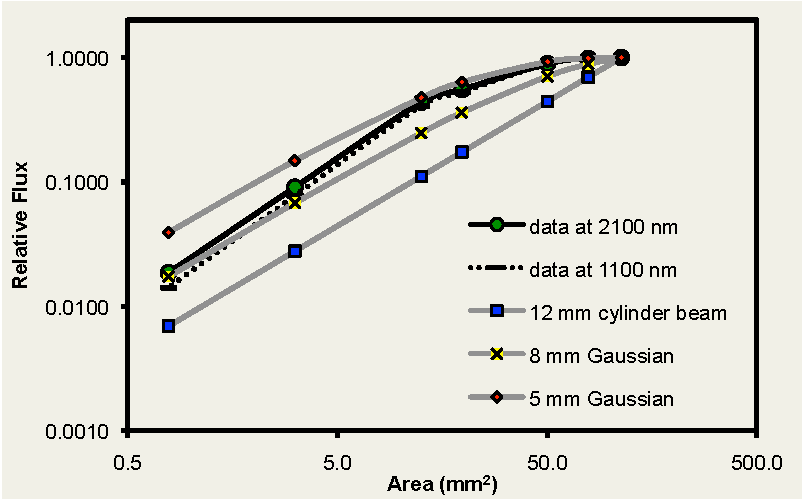
\psfig{file=chFabryPerot/cary5000_beam_notitle.pdf}
\caption[Cary 5000 beam size]{Beam size analysis of the Cary 5000 based on measurements of 7 custom circular apertures.  }
\label{fig:Cary5000beam}
\end{center}
\end{figure}

The measured flux in each band decreases for smaller apertures, conspicuous in Figure \ref{fig:Cary5000beam}.  The slope of the curve of area versus relative flux betrays the beam shape.  An aperture much larger than the beam size will capture all the flux, while apertures comparable or smaller to the beam size will decrease the measured flux.  I modeled three scenarios.  Simplest is a cylindrical beam, also called top-hat profile.  This idealized beam has uniform flux everywhere inside a cutoff radius.  I modeled a threshold radius equal to 12 mm shown in Figure \ref{fig:Cary5000beam} in blue squares.  Another idealized beam profile is a 2 dimensional (2D) Gaussian characterized by a single parameter, its $\sigma$ value.  I modeled $\sigma$ = 8 and 5 mm.  I computed the relative flux of what I called a \emph{truncated Gaussian}, which is the integral:

\scalebox{1.5}{$ f(a, \sigma, b) = \frac{   \int_0^a e^{-r^2/\sigma^2}\,dx    }  {       \int_0^b e^{-r^2/\sigma^2}\,dx      } $}

I set the denominator integral limit $b$ equal to 12 mm, which we know encapsulates all the flux.  The truncated Gaussian models for $\sigma=$ 5 and 8 mm bound the measured data points.  The measured curve follows the 5 mm Gaussian curve and then drops rapidly to meet the 8 mm Gaussian.  I interpret these measurements in the following way.  The real beam shape is something like a fuzzy rectified Gaussian.  That is, the edge of the beam is not sharp, but fuzzy like a 2D Gaussian, but the center is flat topped like the cylindrical beam.  An alternative and equally likely explanation is that the beam is close to a 2D Gaussian, but the custom apertures were not closely aligned with the optic axis.  In either case, the measured FWHM occurred close to the 5 mm circular aperture.

The measured flux in the three spectral bands differs by up to 100 times the measurement uncertainty.  The largest jumps are the positions of known spectral artifacts (cf. Table \ref{tab:C5000Char}) arising from different lamp, filter, and grating configurations.  I interpret the discrepancy as minute spatially-dependent colors within the beam.  This interpretation makes sense- the fine alignment of different optical elements will shift the relative power around within the average beam vector.  This interpretation underscores an important best practice for the Cary 5000.  One must take 100\% baseline spectra with the same aperture as the target spectra.

\subsection{Linearity}

I experimentally measured the Cary 5000 linearity in the following way.  I measured the spectral transmission of 5 neutral density (ND) filters.  I stacked $i$ filters together from total number $N$ = 2 to 5, measuring the stacked spectrum, $T_s$.  I predicted the stacked transmission as: $$T_{p}(\lambda, N) = \prod_{1< i \leq N} T_{i}(\lambda)$$  I computed the mean values of the stacked spectra and predicted spectra.  I assigned an uncertainty of 0.2\% on the mean values, which is the systematic scale error from lamp drift etc.  The 0.2\% lamp drift uncertainty dominates the minuscule uncertainty of the mean.  I propagated the errors on the predicted mean values multiplying the 0.2\% by $N$.  Table \ref{tab:C5000beam} lists the ND filter IDs, predicted mean transmission, measured mean transmission, ratio of measured to predicted, and the discrepancy (in $\sigma$) of the observed minus computed ($O-C$) ratio.  The uncertainty in the ratio is likely underestimated since it merely includes the simple-to-compute lamp drift term.  The low signal to noise measurement of the 5 stacked ND filters likely has a non-negligible contribution from random noise that I have not bothered to quantify.  \texttt{The Right Thing To Do\texttrademark} is to quantify the error attributable to random error and add it in quadrature with my existing error attributable to the 100\% baseline (i.e. lamp) drift.  With this proviso, I ignore the result that the the $O-C$ discrepancy at -24 dB is $3.7\sigma$, assuming that this discrepancy would go away had I performed proper error propagation.  I therefore conclude that the measured and predicted mean transmission are indistinguishable down to 24 dB.


\begin{longtable}{ccccc}
    \caption[Cary 5000 linearity]{Cary 5000 measured linearity} \label{tab:C5000beam} \\
    \hline
      ND stack &  \multicolumn{2}{c}{Mean Transmission} & $T_s/T_p$ & $O-C$ \\  \cline{2-3}
     Sequence & Predicted  &  Measured & Ratio & $\sigma$\\
         \hline
2,3		&	0.2767	&	0.2774	&	1.003	&	0.4\\
2,3,4	& 	0.1369	&	0.1381	&	1.009	&	1.1\\
2,3,4,5	& 	0.0312	&	0.0318	&	1.019	&	1.9\\
2,3,4,5,1&	0.0040	&	0.0042	&	1.044	&	3.7\\
    \hline
\end{longtable}

\begin{figure}[h!] 
\begin{center}
\ 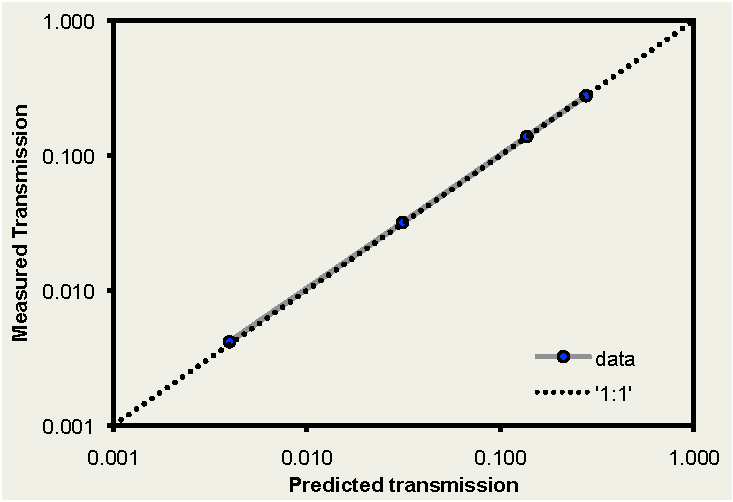
\psfig{file=chFabryPerot/cary5000_linearity_notitle.pdf}
\caption[Cary 5000 linearity plot]{This figure demonstrates the high degree of linearity of the Cary 5000.  The measured value is indistinguishable from the predicted value down to 24 dB.  The error bars are plotted but are imperceptible from the symbols.  There is a minuscule and likely negligible excess of measured flux at the lowest flux measurements.}
\label{fig:Cary5000linearity}
\end{center}
\end{figure}

\subsection{Incidence angle dependence, polarization, and non-standard operation}

It is still not known why the transmission of silicon exceeds the predicted Fresnel reflection value.  I approached this problem in another way, by attacking the angular dependence of the Fresnel equation.  Specifically, the transmission as has a predictable dependence on wavelength and incidence angle.  The extent to which the measured transmission disagrees with the predicted angular dependence could betray the source of the normal-incidence discrepancy.  Non-normal incidence has the feature and problem that it is polarization sensitive.  Polarization makes measurements at non-normal incidence more challenging since the Cary 5000 does not operate by default with polarizers and depolarizers.  Agilent offers a custom polarizer and depolarizer attachment.  Figure \ref{fig:Cary5000Polarizer} shows the light path of the non-standard polarization mode.

\begin{figure}[h!] 
\begin{center}
\ 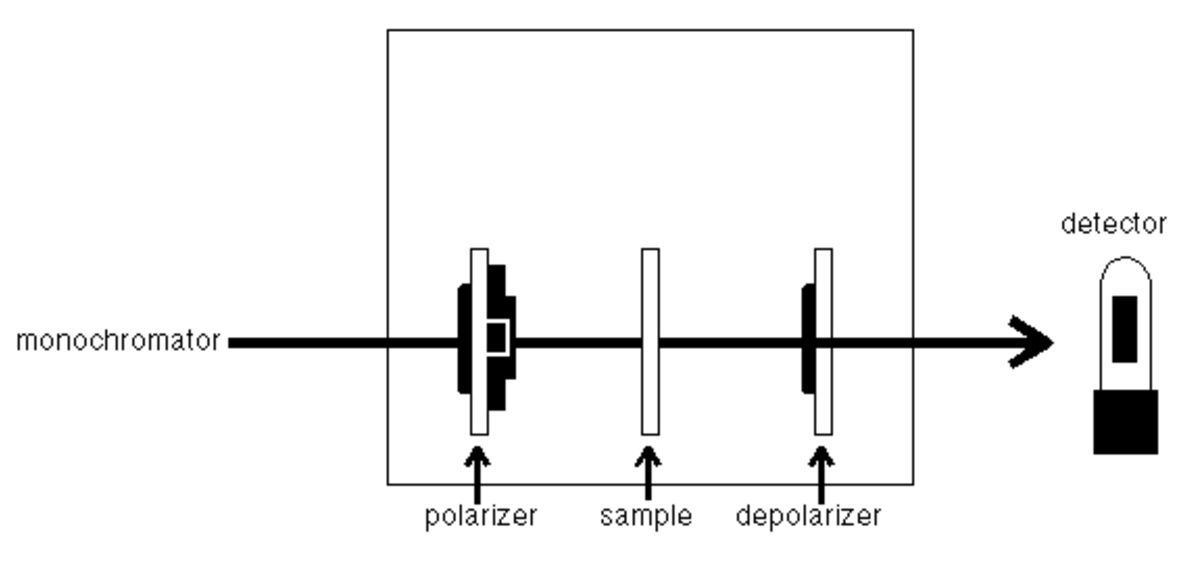
\psfig{file=chFabryPerot/Cary5000polarizer.pdf, width=\textwidth}
\caption[Cary 5000 Polarizer Setup]{Schematic of the Cary 5000 setup to handle polarizing samples.  The graphic is from the Cary 5000 Polarization mode data sheet, which is reprinted in its entirety in Appendix section \ref{sec:A2Cary5000Pol}}
\label{fig:Cary5000Polarizer}
\end{center}
\end{figure}

I measured transmission from $0^\circ - 60^\circ$ incidence angles with no polarizer or depolarizer, and no aperture.  The rotation axis was through the part VG05, on the axis perpendicular to the beam and parallel to the optical bench.  I pitched the top side towards the exit aperture.  I scrutinized the beam path to make sure that the tilted silicon was blocking the entire pupil.  Still, the alignment was challenging, and it is conceivable that the largest incidence angles suffer from light leaks.  The sample holder vignetted the beam at incidence of 60$60^\circ$, so that measurement is excluded from all analysis.

Figure \ref{fig:AngularSiTrans} shows the measured transmission as a function of incidence angle though part VG05, compared to a simple model of Fresnel transmission, assuming an unpolarized incidence beam.  The model and measurements both have samples at a short, moderate, and long wavelength.  The problem at zero incidence angle is apparent-- there is a $\sim50\sigma$ offset between the predicted and measured values.  The offset magnitude and direction remains for 10$^\circ$ incidence.  Measurements beyond 10$^\circ$ show spectral profiles indicative of measurement artifacts from polarization.  For this reason, measurements above 10$^\circ$ can be considered garbage data until we install a measurement approach robust against polarization.

\begin{figure}[h!] 
\begin{center}
\ 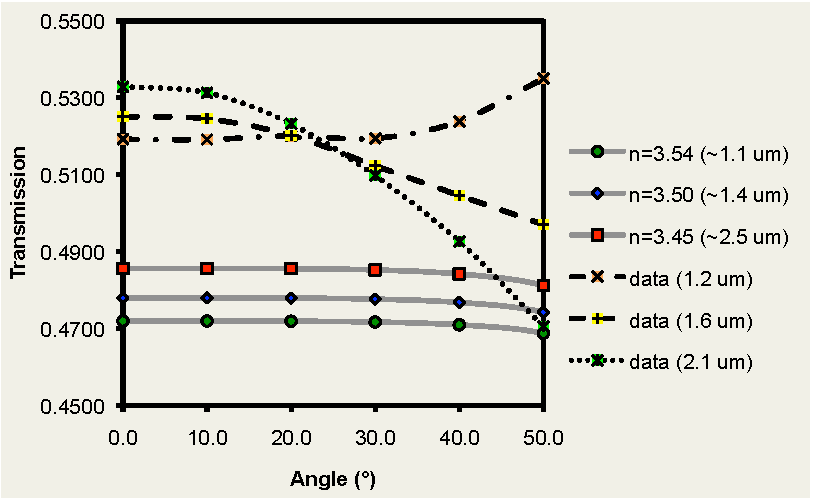
\psfig{file=chFabryPerot/SiTransAng_notitle.pdf, width=\textwidth}
\caption[Angular dependent Si transmission]{Angular dependent Si transmission as measured by the Cary 5000 (top dashed or dotted curves), and predicted from Fresnel transmission theory for unpolarized incident light (bottom gray curves).}
\label{fig:AngularSiTrans}
\end{center}
\end{figure}


\subsection{Fabry-P\`erot analysis for small beam sizes} 
How small of a beam can we use for the Fabry-P\`erot setup?  
I measured the transmission through the 4 $\mu$m cavity in VG03.


\subsection{Multiple incoherent reflections}

Multiple incoherent reflections explain the measured surplus flux over the naive two-surface Fresnel prediction.  The equation for the net transmitted flux through a DSP Si slab, $T_{DSP}$, with $R$ the normal-incidence Fresnel reflection at a single interface and $T=1-R$ the normal-incidence Fresnel transmission:
\begin{eqnarray}
T_{net}=T^2 \sum_{i=0}^{N}R^{2i} \label{eqn:multsum}
\end{eqnarray}
Both $R$ and $T$ are functions of the refractive index, and therefore a function of wavelength and to a much lesser degree, temperature. I had overlooked multiple incoherent reflections by assuming $\sum_{i=0}^{N}R^{2i} \sim 1$ and therefore that $T_{DSP}\sim T^2 $.  The value $N$ is formally infinite, but in practice our measurement error exceeds terms above $N>3$.  For example, the values of the terms $R^{2i}$ for $R= 0.3$ and $i=0-4$ are 1.0, 0.09, 0.0081, 0.0007, and 0.0001.  Compare those values to our measurement errors- assuming purely statistical error, $\sigma=0.0002$; systematic error $\sigma_{sys}=0.002$.  Figure \ref{fig:SiMultFresnel} below graphically illustrates the success of modeling multiple incoherent internal reflections inside the Si wafer.  

\begin{figure}[h!] 
\begin{center}
\ 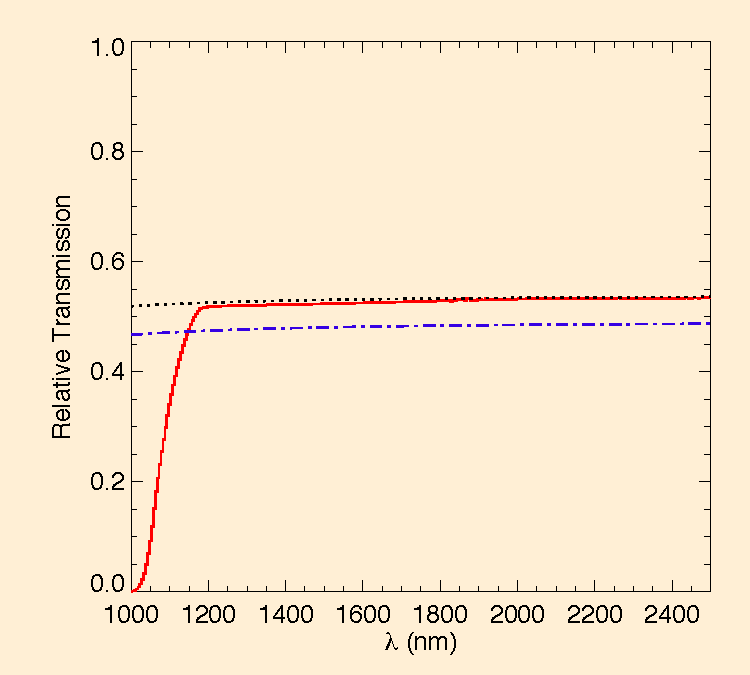
\psfig{file=chFabryPerot/20130502_mult_fresnel.pdf}
\caption[Multiple incoherent internal reflections in a Si puck]{Multiple incoherent internal reflections in a Si puck with parallel surfaces.  The red curve is the transmission spectrum of DSP Si wafer VG05 at normal incidence measured with the Cary 5000.  The blue dash-dot curve is the modeled Fresnel transmission spectrum ignoring multiple internal reflections.  The black dotted line matches the measured transmission spectrum much better because the black dotted line includes multiple internal reflections within the Si wafer.  The measurement error is comparable to the thickness of the line in this high signal to noise measurement.  Still, there is evidence for a dearth of measured flux compared to the prediction with multiple reflections.  The amplitude of the flux deficit ranges from $1-6\; \sigma$ (with $\sigma=\sigma_{sys}=0.002$ from $\lambda=$ 2500 $-$ 1100 nm.  The wavelength dependence hints at scattered light as the origin.}

\label{fig:SiMultFresnel}
\end{center}
\end{figure}

\subsection{Wave transfer matrix approach to computing the emergent transmission spectrum}

In the previous subsection we derived the net transmission through a thick DSP Si slab by directly summing the multiple incoherent reflections (equation \ref{eqn:multsum}).  The problem becomes more complicated when there is a Fabry-P\`erot etalon between the thick DSP Si slab sidewalls.  In this section I explain the mathematical technique to accurately compute the emergent transmission spectrum.  Specifically, there are dozens of permutations of reflection and transmission at each interface that will all contribute  to the emergent spectrum.  For example, a beam can pass through the first Air-Si interface then have the option of transmitting through the Etalon or reflecting.  The transmitted beam can then reflect or transmit through the last Si-Air interface, meanwhile the reflected beam can reflect or transmit through the first Air-Si interface.  In this way, the number of terms that must be summed grows to the power of $n$ where $n$ is the number of passes through the system.  Thankfully, there is a convenient mathematical technique that avoids directly computing each term.  The wave transfer matrix method is described in detail in chapter 7 by Saleh and Teich in ``Fundamentals of Photonics'' \cite{2007SalehTeich}.  Briefly, their technique is to assemble a 2$\times$2 scattering matrix $\boldsymbol{S}$ which has the elements:
\begin{eqnarray}
\boldsymbol{S} = \left(
\begin{array}{cc}
 t_{12} & r_{21} \\
 r_{12} & t_{21} \\
\end{array}
\right)
\end{eqnarray}
Where $t$ and $r$ stand for transmission and reflection respectively.  The order of subscripts is the order of origin and destination of the wave in regards to the interface, so we know something about the direction of the wave and how it got there.  The $\boldsymbol{S}$ matrix encapsulates all the information we need to know about how light waves interact with the interface.  The real power of the matrix technique comes from a cousin of the scattering matrix, the so-called wave transfer matrix, $\boldsymbol{M}$.  The matrix $\boldsymbol{M}$ has the convenient property that its output can be used as the input for another matrix.  In other words, the input vector to $\boldsymbol{M}$ is made of the left and right moving components directly before the interface; the outputs are the left and right moving components directly after the interface:
\begin{eqnarray}
\left(
\begin{array}{c}
 U_2^{(+)} \\
 U_1^{(-)} \\
\end{array}
\right)=\boldsymbol{S} \left(
\begin{array}{c}
 U_1^{(+)} \\
 U_2^{(-)} \\
\end{array}
\right) \\
\left(
\begin{array}{c}
 U_2^{(+)} \\
 U_2^{(-)} \\
\end{array}
\right)=\boldsymbol{M} \left(
\begin{array}{c}
 U_1^{(+)} \\
 U_1^{(-)} \\
\end{array}
\right)
\end{eqnarray}

The elements of $\boldsymbol{S}$ and $\boldsymbol{M}$ are related to each other by geometric transformations\cite{2007SalehTeich}.  Most of the literature on the transfer matrix method deals with applications related to thin films, in which the wavelength is comparable to the size of the dielectric layer.  For thin films the vector components $U_{i}$ represent the complex amplitudes of the electromagnetic waves.  The polarization state can be encapsulated in scattering matrix components\cite{2007SalehTeich}.  The intensities of the emergent spectrum can be computed from the absolute square of the complex amplitudes.  For thick films, the vector components are the intensities of the emergent spectrum, since waves are incoherent.  \cite{2002ApOpt..41.3978K} work out the general transfer-matrix method for optical multilayer systems with incoherent interference.  The key idea for the incoherent transfer matrix method approach is to populate a scattering matrix with elements equal to the (wavelength dependent) transmitted $T_i$ and reflected $R_i$ intensities of an interface or set of interfaces that act together.  Then, use the geometric transformations to construct the $\boldsymbol{M}$ matrix.  

The matrix for the Fabry-P\`erot etalon is calculated in the following way.  The first key idea is that I had to treat the entire air gap as an abstraction, a Fabry-P\`erot etalon.  We don't need to bother to consider the microscopic coherent interactions with the etalon transmission, all of that information is encapsulated in Equation \ref{eq:FabPerot}.  The coefficient of Finesse $F$ and the phase $\delta$ are the two parameters of the Fabry-P\`erot etalon.  The coefficient of Finesse encapsulates the Fresnel reflection and depends only on the Si refractive index which has a minute wavelength (and temperature) dependence.  The phase depends on the wavelength $\lambda$ and $d$ the air gap spacing: $\delta=\frac{2\pi}{\lambda}2d$ .  We assume the etalon is lossless, i.e. the etalon has no absorption $T_e+R_e=1$.  So the incoherent scattering and transfer matrices for the etalon are:

\begin{eqnarray}
\boldsymbol{S_e}&=&\frac{1}{1+F\sin^2{\delta/2}} \left(
\begin{array}{cc}
1 & F \sin ^2(\delta/2) \\
F \sin ^2(\delta/2) & 1 \\
\end{array}
\right) \nonumber \\
\nonumber \\
\boldsymbol{M_e}&=&\left(
\begin{array}{cc}
 1-F \sin ^2(\delta/2) & F \sin ^2(\delta/2) \\
 -F \sin ^2(\delta/2) & 1+F \sin ^2(\delta/2) \\
\end{array}
\right)
\label{eqn:EtalonMatrix}
\end{eqnarray}

I assembled the matrix for the Air-Si Fresnel interface in the following way.  First it is important to note that the matrix is the same whether the transmission is from Si to air or air to Si.  This reciprocity is not necessarily true for the complex amplitudes matrix, but our approach employs intensities not complex amplitudes.  The Fresnel interface is lossless.  The transmission and reflection are given by the Fresnel equation for normal incidence:
\begin{eqnarray}
T_n&=&\frac{4n_{Si}}{(n_{Si}+1)^2} \\
R_n&=&\frac{(n_{Si}-1)^2}{(n_{Si}+1)^2} \label{eq:FresnelTrans}
\end{eqnarray}
For clarity I will drop the subscripts from $n_{Si}$, since we have already set $n_{air}=1$ and there are no other dielectric interfaces to think about.  So the scattering and transfer matrices for the air-Si Fresnel boundary are:

\begin{eqnarray}
\boldsymbol{S_n}&=&\frac{1}{(n+1)^2} \left(
\begin{array}{cc}
4n & (n-1)^2 \\
(n-1)^2 & 4n \\
\end{array}
\right)  \nonumber \\
\nonumber \\
\boldsymbol{M_n}&=&\frac{1}{4n}\left(
\begin{array}{cc}
 -n^2+6  n-1 & ( n-1)^2 \\
 -( n-1)^2 & ( n+1)^2 \\
\end{array}
\right)
\label{eqn:SiAirMatrix}
\end{eqnarray}

Finally, we cascade the matrices together to compute the net transmission through the stack of abstractions.  The result is a $2\times2$ transfer matrix: $$\boldsymbol{M_{net}}=\boldsymbol{M_n}\boldsymbol{M_e}\boldsymbol{M_n}$$  From the matrix transformation equations \cite{2007SalehTeich} we know $M_{22}=1/T$.  Taking the inverse of the bottom right element of $\boldsymbol{M_{net}}$, we get the transmission $T_{net}$ through the net optical device: 

\begin{eqnarray}
T_{net}=\frac{2 n}{1+ 2n F\sin ^2(\delta/2)+n^2} \label{eqn:FPmatTrans}
\end{eqnarray}

Compare equations \ref{eqn:FPmatTrans} and \ref{eq:FabPerot}.  The revised transmission has picked up a few factors of 2 and $n$.  While we are at it, let's compute the matrix for the scenario with no intermediate etalon: there are simply two Fresnel interfaces with which light interacts incoherently.  This scenario is the model for a single DSP reference puck. The revised matrix multiplication is simply $\boldsymbol{M_{DSP}}=\boldsymbol{M_n}\boldsymbol{M_n}$.  Taking the inverse of the $M_{22}$ element, we find: 
\begin{eqnarray}
T_{DSP}=\frac{2 n}{n^2+1}\label{eqn:EqofSummedSlab}
\end{eqnarray}
which is apparently equal to Equation \ref{eqn:multsum}!